\documentclass[sn-mathphys-num]{sn-jnl}

%%%% Standard Packages
%%<additional latex packages if required can be included here>

\usepackage{graphicx}% 
\graphicspath{ {./Images/} }
\usepackage{enumerate}
\usepackage[dvipsnames,table]{xcolor}
\usepackage[most]{tcolorbox}
\usepackage{array}
\usepackage{amsmath} % For Piecewise Functions
\usepackage{breqn} % To Split Long Equations
\usepackage{enumitem} % For Bracketed Numbers in References
\usepackage[absolute,overlay]{textpos} % For Side Axes Label in Table
\usepackage{float} % To Position Table Accurately

\usepackage{multirow}%
\usepackage{amsmath,amssymb,amsfonts}%
\usepackage{amsthm}%
\usepackage{mathrsfs}%
\usepackage[title]{appendix}%
\usepackage{xcolor}%
\usepackage{textcomp}%
\usepackage{manyfoot}%
\usepackage{booktabs}%
\usepackage{algorithm}%
\usepackage{algorithmicx}%
\usepackage{algpseudocode}%
\usepackage{listings}%
%%%%

%% As per the requirement new theorem styles can be included as shown below
\theoremstyle{thmstyleone}%
\newtheorem{theorem}{Theorem}%  meant for continuous numbers
%%\newtheorem{theorem}{Theorem}[section]% meant for sectionwise numbers
%% optional argument [theorem] produces theorem numbering sequence instead of independent numbers for Proposition
\newtheorem{proposition}[theorem]{Proposition}% 
%%\newtheorem{proposition}{Proposition}% to get separate numbers for theorem and proposition etc.

\theoremstyle{thmstyletwo}%
\newtheorem{example}{Example}%
\newtheorem{remark}{Remark}%

\theoremstyle{thmstylethree}%
\newtheorem{definition}{Definition}%

\raggedbottom
%%\unnumbered% uncomment this for unnumbered level heads

\begin{document}

% Title 
\title[Article Title]{\centering Decentralizing the Odds:\\ A Peer-to-Peer Alternative to the Money Line}

\author*{\fnm{Jacob} \sur{Wyngaard}}
\affil{\orgdiv{Department of Mathematics}, \orgname{University of Delaware}, \orgaddress{\street{Ewing Hall}, \city{Newark}, \postcode{19716}, \state{DE}, \country{USA}}} % Get Permission to Use This

 \email{jakewyn@udel.edu}


%%==================================%%
%% Sample for unstructured abstract %%
%%==================================%%

\abstract{Contemporary peer to peer (P2P) betting revolves around betting exchanges, where players place and lay bets in a marketplace supervised by the P2P sportsbook. In this paper, I introduce a novel system of P2P gambling, where the sportsbook takes a more active role in bet creation. Within this system, users submit their subjective probabilities and bet amounts regarding a binary event outcome. Bet amounts are partitioned into slices, which are matched with the slices of other players into peer bets. The stakes, win conditions, and payouts of each peer bet are assigned to provide both players with an equivalent and positive expectation value, according to their corresponding subjective probabilities. Sportsbooks profit by taking a rake from each peer bet pot, in proportion to the amount of subjective expectation created. Residual bet amounts are engaged in an iterative series of money lines, generating additional subjective expectation for the users and additional profit for the sportsbook. This integrated approach, designated the synthesized speculation gambling system, ensures that sportsbook profit is invariant regarding the binary event outcome. My research analyzes the production of user subjective expectation and sportsbook profit through the synthesized speculation system across varying distributions of user subjective probability and betting capacity, in direct competition with the traditional money line. Through this analysis, this paper demonstrates that the synthesized speculation gambling system increases both user subjective expectation and sportsbook profit relative to the traditional money line system. My paper concludes with the recommendation of the synthesized speculation system as a supplement to the traditional money line, as a method of informed speculation for binary events with particular probability spaces.}

\keywords{Gambling, Peer-to-Peer, Subjective Probability, Computational Modeling}

\maketitle

% Starting the Sections

\section{Background}

\subsection{Money Lines}

The gambling considered within this paper will be limited to binary events, such as the winner of an NFL playoff game. The outcome space of a binary event is dualistic, consisting of a focal outcome and a compliment outcome. Currently, the predominant method of gambling on binary events is the money line. The money line maps each binary event outcome to its American odds. American odds are expressed in the following convention: $-N$ implies that for every $N$ dollars you bet on that outcome, you will receive 100 dollars if that outcome occurs. $N$ implies that for every 100 dollars you bet on that outcome, you will receive $N$ dollars if that outcome occurs. Since N is at least 100 by convention, a negative number implies a win probability greater than half unity, while a positive number implies a win probability below half unity. 

For most money lines, one binary event outcome is considered probable enough to have negative odds, while the other outcome is considered improbable enough to have positive odds. In this case, the outcome with negative odds is classfied as the favorite and the outcome with positive odds is classified as the underdog. In the money line below, I denote the favorite odds with $-\alpha$ and the underdog odds with $\beta$. This notation will be used for the remainder of this section.

% Money Line Table - Start
\newcolumntype{C}[1]{>{\centering\arraybackslash}m{#1}}
\renewcommand{\arraystretch}{3.8}
\setlength\extrarowheight{-.07cm}
%

\begin{center} 
	\begin{table}[h]
	\centering
	\begin{tabular}{ | C{6 cm} | C{6 cm} | }
	\hline
	\cellcolor{Salmon} \large Favorite & \cellcolor{lightgray} \large -$\alpha$  \\ 
	\hline
	\cellcolor{YellowGreen} \large Underdog & \cellcolor{lightgray} \large +$\beta$  \\  
	\hline
	\end{tabular}
	\caption{The Money Line}
	\end{table}
\end{center}
\vspace{-15pt}
% Money Line Table - End


If both binary event outcomes have approximately the same chance of occuring, both are assigned negative odds, typically around $-110$ (Andrews, 2019; Walters, 2023). If this is the case and there is equivalent betting action on both outcomes, the sportsbook makes a vigorish of $4.5\%$, which is the conventional sportsbook profit margin (Action Network, 2019; Walters, 2023). I assume that the objectives of the sportsbook when laying a money line are two-fold: to generate a proportioned balance of bets on the outcomes and to produce a profit via overrounds (setting $\alpha > \beta$). In reality, sportsbooks may forgo balance and skew the bet equilibrium towards the outcome that they consider the most overpriced (Andrews, 2019; Levitt, 2004). For the purposes of this paper, however, sportsbooks are assumed to prioritize proportionately balancing bets before they optimize for profit.

\subsection{Gambler's Perspective}

This paper assumes that each player has a subjective probability $p$ that corresponds to their degree of belief in the focal outcome. These subjective probabilities are assumed to vary across the gambling population, as a result of differences in personal experience and heuristic. As Schr\"{o}dinger wrote, probability is never computed in vacuum but instead "in regard to a certain given state of knowledge" (1947). Estimating the distribution of subjective probability is an active research area (Andersen et al., 2014), as is the evolution of subjective probability via Bayesian learning (Alós-Ferrer and Mihm, 2023; von Holstein, 1971). However, those research topics lie beyond the scope of this paper. I assume that each player has an individual subjective probability, and that this subjective probability is static upon contact with the money line. In the remainder of this section, let's assume that the distribution of subjective probabilities is clustered above half unity, enough for the focal outcome to be relabeled the favorite outcome. Accordingly, the compliment outcome is relabeled the underdog outcome. Bettors are assumed to act rationally in that they will only bet on outcomes that generate a non-negative expectation value according to their subjective probability. If $p_{\alpha}$ is defined as the minimum subjective probability for betting on the favorite and $p_{\beta}$ is defined as the maximum subjective probability for betting on the underdog, this assumption of rationality produces the following results:

\begin{equation}
 p_\alpha = \frac{\alpha}{\alpha + 100}      
\end{equation}

\begin{equation}
p_\beta= \frac{\beta}{\beta + 100}      
\end{equation}
\vspace{.05in}

If $\alpha = \beta$, all subjective probabilities $p$ have an available money line bet with a non-negative subjective expectation value. However, given that money lines require $\alpha > \beta$ in order to be profitable, there exists subset of subjective probabilites, a no man's land of $p_{\beta} < p < p_{\alpha}$, in which betting on either outcome has a negative subjective expectation value. The difference between $\alpha$ and $\beta$ can be conceptualized as the gambling equivalent to the bid-ask spread in financial trading.

\subsection{Making the Money Line}

This paper assumes that, when sportsbooks make their money lines, they do so with knowledge of each consumer's subjective probability (denoted $p_{i}$) as well as the amount of money each consumer is willing to bet (denoted $m_{i}$). These values can be envisioned as the binary event equivalent of the $p_{ij}$ and $\beta_{ij}$ matrices used by Eisenberg and Gale in their seminal paper on consensus in pari-mutuel gambling (1959). This information can be consolidated into a money density function $\rho_M(p)$. This function is the amount of money willing to be bet as a function of subjective probability. For example, if $\rho_M(.5)$ = \$100, then the total amount of money willing to be bet by people who believe that the focal outcome has a 50\% chance of occuring is \$100. The construction of $\rho_M(p)$ from the individual $m_i$'s and $p_i$'s is as follows:

\begin{equation}
\rho_M(p) = \sum_{i}
   \begin{cases} 
     0 & p_i \neq p \\
     m_i & p_i = p \\
   \end{cases}
\end{equation}

Additionally, I define the cumulative money density function $\Gamma(p)$:
\begin{equation}
\Gamma(p) = \int_0^p\rho_M(p') dp'
\end{equation}

Using this construction, the sportsbook can compute its profit under either binary event outcome: 

\begin{center}
\underline{\textbf{Favorite Wins}}
\end{center}

\begin{equation}
\textnormal{Sportsbook Profit} = \Gamma(p_\beta)-\frac{100}{\alpha}(\Gamma(1)-\Gamma(p_\alpha)) 
\end{equation}
\vspace{.05in}

\begin{center}
\underline{\textbf{Underdog Wins}}
\end{center}

\begin{equation}
\textnormal{Sportsbook Profit} =  (\Gamma(1)-\Gamma(p_\alpha)) - \frac{\beta}{100} \Gamma(p_\beta)
\end{equation}
\vspace{.05in}

By previous assumption, the money line is created such that the vigorish is maximized while remaining invariant to the binary event outcome. The $p_\alpha$ and $p_\beta$, and therefore the $\alpha$ and $\beta$ of the moneyline, that accomplish this can be found by applying the Lagrange multipliers method to a constraint function representing balance and an objective function representing profit. Now, the Lagrange multipliers method requires that $\rho_M$ is continuous across the subjective probability domain $[0,1]$. In situations with large numbers of players, $\rho_M$ can be reasonably assumed to fulfill this condition. The constraint equation $C(p_\alpha,p_\beta)$ is constructed by setting the difference between Equation (5) and Equation (6) equal to zero, while the objective function $P(p_\alpha,p_\beta)$ is simply Equation (6).

\begin{equation}
C(p_\alpha,p_\beta) := \Gamma(p_\beta) - \frac{100}{\alpha}(\Gamma(1)-\Gamma(p_\alpha)) - (\Gamma(1)-\Gamma(p_\alpha)) + \frac{\beta}{100}\Gamma(p_\beta) = 0
\end{equation}

\begin{equation}
P(p_\alpha,p_\beta) := (\Gamma(1)-\Gamma(p_\alpha)) - \frac{\beta}{100}\Gamma(p_\beta)
\end{equation}
\vspace{.05in}

Using the constraint function and the defintions of $p_\alpha$ and $p_\beta$, $C(p_\alpha,p_\beta)$ and $P(p_\alpha,p_\beta)$ can be simplified into the folllowing:

\begin{equation}
C(p_\alpha,p_\beta) := p_\alpha \Gamma(p_\beta) - (1-p_\beta)(\Gamma(1)-\Gamma(p_\alpha)) = 0
\end{equation}

\begin{equation}
P(p_\alpha,p_\beta) := (1-\frac{p_\beta}{p_\alpha})(\Gamma(1)-\Gamma(p_\alpha))
\end{equation}
\vspace{.05in}

Employing the Lagrange multiplier method with Equations (9) and (10), I derived a necessary condition. This condition, defined in Equation (12), is an additional requirement to the constraint function's equivalence to zero. Consequently, the money line which maximizes profit while maintaining balanced outcomes must fulfill the following two conditions: \\

\begin{equation}
p_\alpha \Gamma(p_\beta) - (1-p_\beta)(\Gamma(1)-\Gamma(p_\alpha))  = 0
\end{equation}

\begin{equation}
\begin{split}
p_\alpha (1-p_\alpha) \rho_M(p_\alpha) \Gamma(p_\beta) + p_\beta (1-p_\beta) \rho_M(p_\beta) (\Gamma(1)-\Gamma(p_\alpha))  \hspace{10pt}\\
+ \Gamma(p_\beta)(\Gamma(1)-\Gamma(p_\alpha)) - (p_\alpha - p_\beta) p_\alpha (1 - p_\beta) \rho_M(p_\alpha) \rho_M(p_\beta) = 0
\end{split}
\end{equation}

Therefore, if the sportsbook knows the money density function $\rho_{M}(p)$ (and thus $\Gamma(p)$), the sportsbook can create a money line which optimizes sportsbook profit under the constraint of balanced outcomes. 

\subsection{Money Line Limitations}

While the money line has existed as profiable gambling appartus since the mid-20th century (Schwartz, 2006), it has three significant limitations:
\vspace{.05in}
\begin {enumerate}
\vspace{.05in}
\item \textbf{Limited Customer Base}
\vspace{.05in}
\\Customers with a subjective probability $p$ in the no man's land of $ p_\beta < p < p_\alpha$ have no possible bets with non-negative subjective expectation. Additionally, in order to preserve balanced outcomes, sportsbooks may severely limit bets placed by professional sports bettors. Billy Walters, a professional gambler who has bet hundreds of millions of dollars over the course of his career, famously hired dozens of "beards" to covertly place bets for him to circumnavigate these limits (Walters, 2023). 

\vspace{.05in}
\item \textbf{Balance Uncertainty}
\vspace{.05in}
\\This section assumed that the sportsbook knows $\rho_M(p)$. In reality, there is enough uncertainty with customer betting patterns that sportsbooks may unintentionally take a disproportionate share of bets on one event outome. This can have disastrous consequences, such as in 1946 when Airborne, a fan favorite with 50 to 1 odds, won the Epsom Derby and drove over half of Britain's bookmakers into bankruptcy (Smith, 2002). 

\vspace{.05in}
\item \textbf{Lack of Customer Differentiation}
\vspace{.05in}
\\Customers with $p >> p_\alpha$ receive the same odds for betting on the favorite as customers with $p = p_\alpha$. Likewise, customers with $p << p_\beta$ receive the same odds for betting on the underdog as customers with $p = p_\beta$. Even if their payouts were decreased, customers with extreme subjective probabilities relative to the $p_\alpha$ and $p_\beta$ would still have bets with positive subjective expectation and would therefore still be expected to place bets with the money line. Thus, by treating customers of all subjective probabilities the same, the sportsbook overpays the winning customers with extreme subjective probabilities.
\end{enumerate}

\section{Betting Exchanges}

The current implementation of peer to peer gambling is the betting exchange. Companies such as Sporttrade, Prophet Exchange, and BettorEdge follow this approach, allowing users to lay their own money lines and to bet on the money lines laid by other users. Competition within these markets, combined with the low barrier to entry of posting a money line, drive $\alpha$ and $\beta$ closer together within the user moneylines. According to a 2022 ESPN article, money lines posted on Sporttrade and Prophet Exchange at the start of the 2022 NFL season provided more favorable odds than those of traditional sportsbooks (Purdum). Betting exchange profit, the article claims, is acquired by taking a commision approximately equal to two percent of the winning player's net earnings. BettorEdge follows a different business model, making money from advertising, premium subscriptions, and processing fees on certain orders (BettorEdge, 2024). Within these gambling architectures, the betting exhange functions as the host of the money line marketplace without acting in the traditional market maker capacity of a sportsbook. This allows the betting exchange to avoid the balance uncertainty of traditional sportsbooks while eliminating the need for bookmakering expertise to craft a card of money lines. However, the betting exchange is severely handicapped when it comes to making profit as it only makes a $2\%$ profit margin from winnings, for a total profit margin around $1\%$. As we will see, this drastically underperforms the money line and synthesized speculation gambling system. 

\section{Synthesized Speculation System}

\subsection{Overview}

The synthesized speculation system consists of two components: a peer bet system and an iterative money line. This system collects batches of user subjective probabilities and bet amounts, and returns monetary reward structures for each player for the binary event. These structures are generated first by partitioning bet amounts into slices and placing these slices into the peer bet system, then engaging residual bet amounts via an iterative money line. I would like to note that the synthesized speculation system is by no means the only or even the most profitable gambling system that could be constructed from the elements of this section. One possible alternative is a system that gathers the residual money into slices and creates more peer bets before conducting the iterative money line. Another would implement the iterative money line first and then perform peer to peer gambling in no man's land. It is hoped that this paper will stimulate interest in the creation and application of such novel gambling systems.

\subsection{Motivation of Peer Bet System}

This paper will introduce a novel peer to peer gambling system which, while similar to betting exchanges in that it guarantees balance, increases sportsbook profit by taking a more active role in user matching. The motivation for this system is the rental harmony problem, which attempts to create envy-free assignments of rooms and rental payments among a group of housemates. Using Sperner's lemma and a simple set of assumptions, it can be shown that there must always exist at least one envy free solution to this problem (Su, 1999).  In a two housemate rental harmony problem, an envy-solution can be generated by by querying each housemate for the value of one bedroom, and assigning that room to whoever valued it the most  (Malone and Herships, 2019). The rental payment for that room is simply the average of the provided values, with the other room's rent the remainder of the total house rent. Rental harmomy can be mapped to peer betting via the replacement of room assignment with the binary event win condition, and the rental payment with betting odds. 

\subsection{Overview of Peer Bet System}

Users will be given a focal outcome of a binary event (such as the home team winning an NFL playoff game) and queried for their subjective probability regarding this outcome. Users's bet amounts will be partitioned into slices, which will be matched with each other into peer bets based on their corresponding subjective probabilities. The ideal matching strategy is an open area of investigation (see Appendix A) and the current convention is to use the simple outside-in matching strategy, discussed further in subsection 3.5. Within each peer bet, the slice with the higher subjective probability will be assigned the focal outcome as a winning condition, with the other slice assigned the compliment outcome as a winning condition. The stakes of each slice are set algebraically such that both slices have the same positive expectation value according to their corresponding subjective probabilities. The maximum stake of either slice is simple the slice value. In this system, the maximum slice stake is set at \$5, and players with bets of $\$B$ will have their bet seperated into $\textrm{floor}(\frac{B}{5})$ different slices, with any remaining money set aside. This system makes a profit by taking a rake from each peer bet pot, with the rake proportional to the subjective expectation value of the slices within that peer bet. Unlike a traditional money line, customers of all subjective probabilities have access to positive subjective expectation bets, except in the extremely unlikely outcome that over half of the slice subjective probabilities are equivalent. Additionally, customers' bets are priced more accurately, so that customers with more moderate (and likely better informed) subjective probabilities receive better odds than customers with more extreme (and likely less informed)  subjective probabilities. This system is designed to reward informed speculation, and because it doesn't require bookmakers, can be applied to any binary event with an unknown probability space.

\subsection{The Peer Bet}

In the table below, the win condition and stake assignment for each slice in a peer bet is given, assuming that the subjective probability of slice 2 (denoted $p_>$) exceeds the subjective probability of slice 1 (denoted $p_<$). Additionally, I assume that the rake taken by the sportsbook is equivalent to some adjustable parameter $\lambda$ times the subjective expectation value (SEV) of either slice. Unless otherwise specified, $\lambda$ will be set to two within this paper.

\pagebreak

% Peer to Peer Table - Start
\newcolumntype{C}[1]{>{\centering\arraybackslash}m{#1}}
\renewcommand{\arraystretch}{3.8}
\setlength\extrarowheight{-.07cm}

\begin{center} 
	\begin{table}[ht]
	\centering
	\begin{tabular}{ | C{4 cm} | C{4 cm} | C{4 cm} |}
	\hline
	& \large Slice 1 & \large Slice 2 \\
	\hline
	\large Probability & \large $p_<$ & \large $p_>$ \\
	\hline
	\large Win Condition & \large Compliment Outcome & \large Focal Outcome \\
	\hline
	\large Stake if $p_< + p_> \leq 1$ & \large 5 & \large $5 \hspace{2pt} \frac{p_<+p_>+p_>\lambda}{2-p_<-p_>+ (1-p_<)\lambda}$ \\
        \hline
	\large Stake if $p_< + p_> > 1$  & \large $5 \hspace{2pt} \frac{2-p_<-p_>+ (1-p_<)\lambda}{p_<+p_>+p_>\lambda}$ & \large 5 \\
        \hline
	\large SEV if $p_< + p_> \leq 1$  & \large $5 \hspace{2pt} \frac{p_>-p_<}{2-p_<-p_>+(1-p_<) \lambda}$ & \large $5 \hspace{2pt} \frac{p_>-p_<}{2-p_<-p_>+(1-p_<) \lambda}$ \\
        \hline
	\large SEV if $p_< + p_> > 1$  & \large $5 \hspace{2pt} \frac{p_>-p_<}{p_<+p_>+p_> \lambda}$ & \large  $5 \hspace{2pt} \frac{p_>-p_<}{p_<+p_>+p_> \lambda}$  \\
        \hline

	\end{tabular}
	\caption{Assignments within a P2P Bet}
	\end{table}
\end{center}
\vspace{-15pt}
% Peer to Peer Table - End

As evident in the table above, subjective expectation value arises from the asymmetry in player subjective probabilities. If $p_< = p_>$, no subjective expectation is created. Like other economic markets, differences in asset valuation (the asset, in this case, being a bet on the focal outcome) drive commerical transactions in which both parties conclude that they have made a profitable trade. This allows the markets to seemingly create value out of nothing, until the proper asset valuation is determined via price discovery. In financial markets, price discovery occurs through the negotiations between buyers and sellers. In gambling, price discovery is simply the occurence of the binary event.

\subsection{Batch, Sort, Match}

This system of peer to peer gambling becomes considerably more complicated as\\N $>>$ 2 players are considered over a large time period before the binary event. The complication is twofold: how to batch players across time and how to match bet slices to maximize both user subjective expectation and sportsbook profit. The temporal problem is generating enough players in a batch while delivering bets in a reasonable timeframe. Higher batch turnover both reduces bet timelines and lessens the information asymmetry between early bettors and late bettors within the same batch. While bet delivery will almost certainly take longer than a traditional money line, providing accurate batching timelines will likely reduce customer dissatisfaction (Maister, 1985). This paper tentatively suggests a batching timeframe of one hour, with more confident recommendations contingent on further research.

The second complication within the peer bet system is how to effectively match bet slices. Before matching, bet slices are sorted into ascending order using their user's subjective probability values. Bet slices are then matched with each other based off this sorting order. There is a massive number of possible matching strategies, none of which strictly dominate across varying subjective probability distributions. However, as shown in Appendix A, the outside-in matching strategy is highly effective yet simple to implement relative to these other strategies. This outside-in matching strategy pairs the slice with the highest subjective probability with the slice with the lowest, the slice with the second highest with the slice with the second lowest, and so on. A batch, sort, match process with outside-in matching is shown in Figure 1. 

\begin{figure}[H]
	\centering
	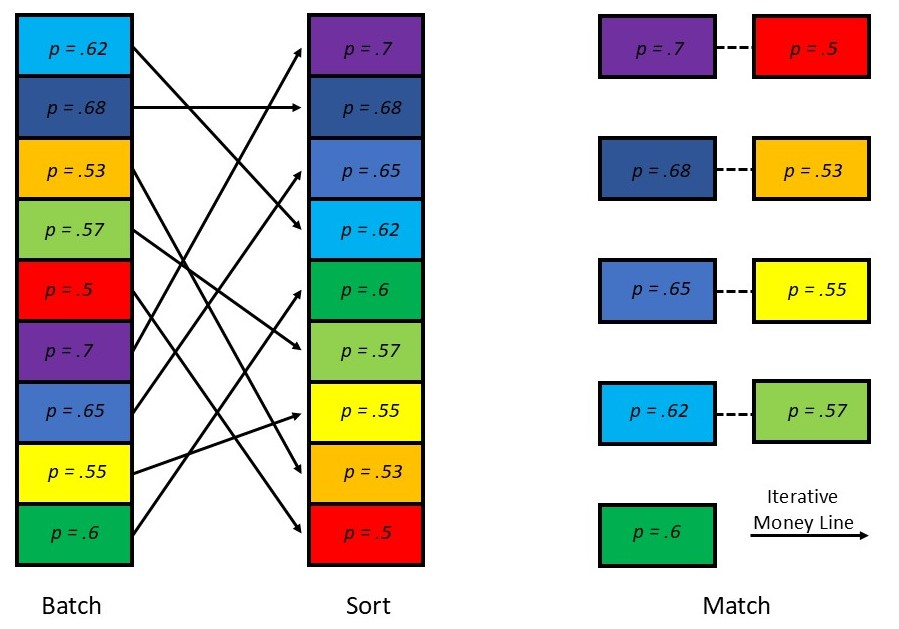
\includegraphics[width=10cm]{Batch Sort Match - IO}
	\caption{Batch, Sort, Outside-In Match}
\end{figure}

\subsection{Iterative Money Line on Residuals}

Unfortunately, solely executing a batch, sort, and match peer bet system leaves plenty of money on the table. As reflected in Table 2, unless $p_< + p_> = 1$, one slice will not be betting with the maximum stake amount. This residual money, along with the residuals from bet slicing, can still be engaged in positive subjective expectation bets that generate sportsbook profit. To accomplish this, I recommend the implementation of an iterative money line across the remaining bet amounts. 

The iterative money line, at its first iteration, is simply a traditional money line (as discussed in Section 1). Whereas a traditional money line sets one pair of odds and accepts the customers in no man's land as a lost cause, the iterative money line continually makes new money lines with the customers in no man's land. This process only stops after a maximum number of iterations or when the marginal profit falls below a given threshold. By setting multiple sets of money line odds, the sportsbook reaches customers that the traditional money line would overlook. Given the obvious differential in odds offered to different customers, the iterative money line would cause considerable backlash if operated as a stand-alone, transparent gambling system. However, in a black box architecture such as the synthesized speculation gambling system, where customers expect the system to provide positive subjective expectation bets, the iterative money line is a great way to boost customer subjective expectation and sportsbook profits. 

\begin{figure}[H]
	\centering
	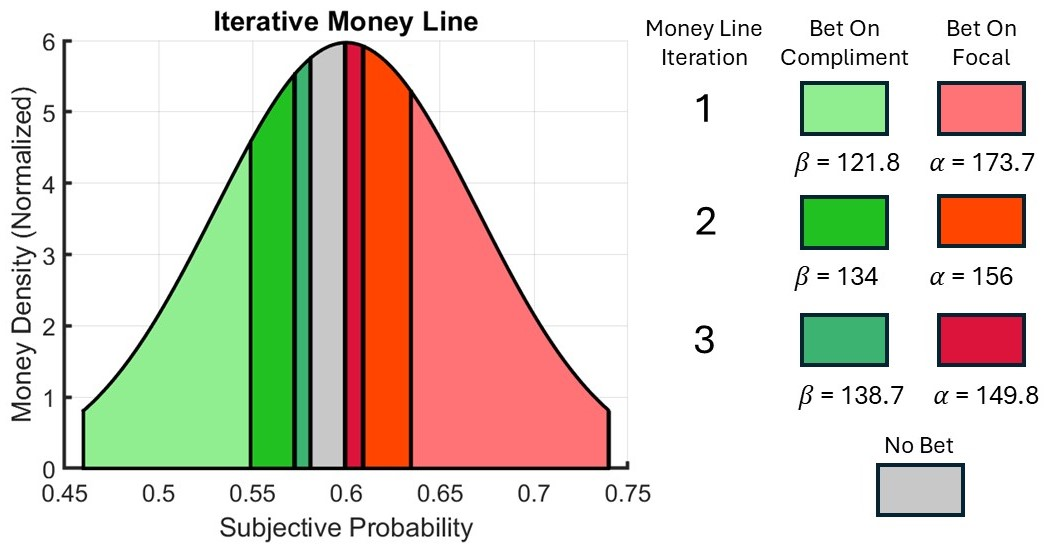
\includegraphics[width=12cm]{Iterative Money Line}
	\caption{Example Iterative Money Line}
\end{figure}

\subsection{Synthesized Speculation Synopsis}

In summary, the synthesized speculation gambling system, the gambling system recommended by this paper, will be comprised of the following operations:

\begin{enumerate}[label=\textbf{\arabic*})]

\vspace{.05in}
\item Input a batch of customer subjective probabilities $p_i$ and betting amounts $m_i$.
\vspace{.05in}

\item Slice each $m_i$ into a discrete amount of \$5 bets, each with the subjective probability $p_i$. Any residual money that doesn't make it into a slice will be set aside, along with its subjective probability, for the iterative money line. 
\vspace{.05in}

\item Sort and match the \$5 slices using the outside-in matching strategy. Assign a win condition, stake, and payout for each slice in the peer bet using the methodology from Table 2. If a slice's stake is less than the \$5 maximum, the residual money will also be set aside for the iterative money line. 
\vspace{.05in}

\item Conduct an iterative money line process using the residual money. Each player will be assigned a win condition, stake, and payout, with the exception of the small minority whose subjective probabilities are in the drastically reduced no man's land.
\vspace{.05in}

\item Combine the peer bet slices and iterative money line bets of each player to give each player their monetary results for both binary event outcomes. For the ith player, $f_i$ denotes the monetary result of the focal outcome and $c_i$ denotes the monetary result of the compliment outcome. Every player will have a positive subjective expectation value, equal to $p_i f_i + (1-p_i) c_i$.
\vspace{.05in}
\end{enumerate}

\begin{figure}[H]
	\centering
	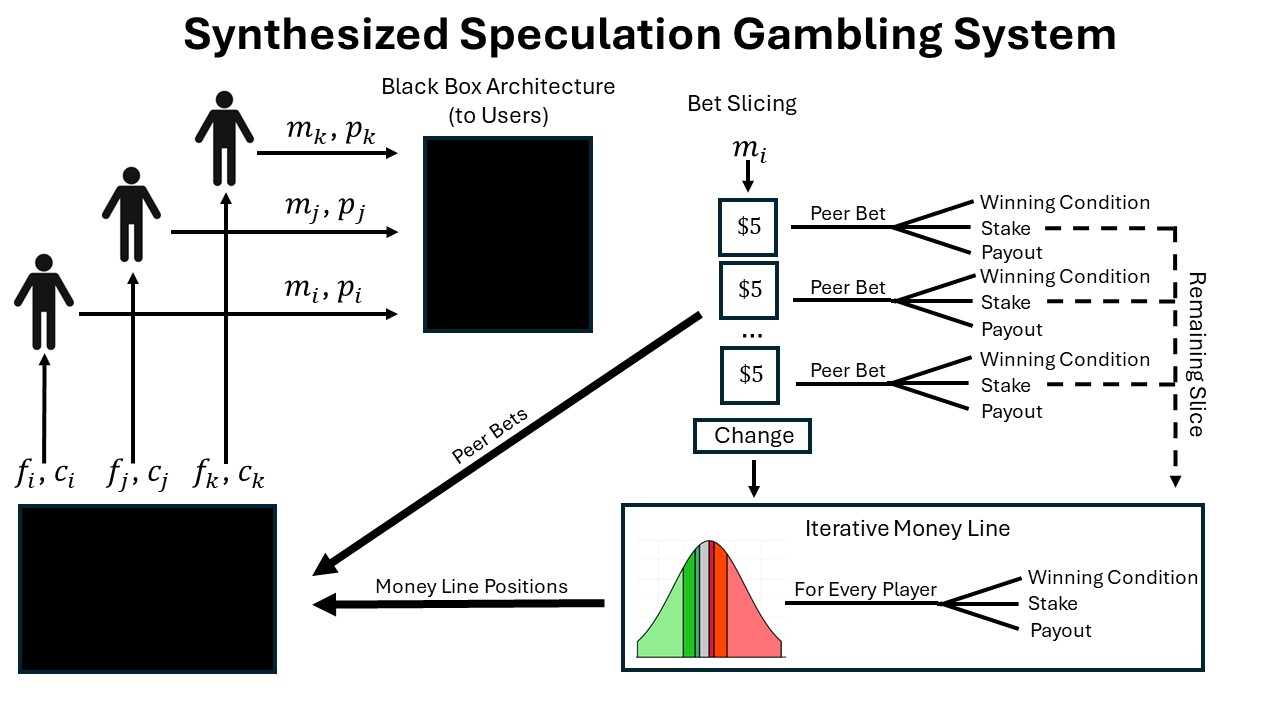
\includegraphics[width=14cm]{Synthesized Speculation Gambling System}
	\caption{Synthesized Speculation Gambling System}
\end{figure}

\section{Methods}

\subsection{Modeling Subjective Probability}

In order to compare customer and sportsbook outcomes between the traditional money line and the synthesized speculation gambling system, we must find a realistic $\rho_M$ to generate sample data from. Data from the Health and Retirement Survey (HRS) illustrate that subjective probabilities for binary questions regarding personal lifespan and retirement age are widely distributed and in some cases, irrational (Hurd and McGarry, 1993). Additional analysis suggests that, at least for the HRS, subjective probabilities tend to cluster around certain responses, especially 50\%. (Hurd, 2011). Another academic study looked at the distribution of subjective probabilities for binary events with the introduction of scoring rules using the actual outcome (Andersen et. al, 2014). For both scoring rules, the subjective probability distributions varied drastically in shape across the binary events in question, with topics ranging from presidential election results to the impact of gender on empathy.

Between these studies, it is evident that while subjective probabilities can cluster around certain values, their overall distribution is unpredictable. Given this unpredictability, this paper will use the beta distribution to model subjective probability due to its popularity as a Bayesian prior probability distribution in academic literature (Taroni et al., 2018; von Holstein, 1971; Wu et al., 2008). However, this paper will make two modfications, the first being the restriction of the distribution domain to $[\frac{1}{4}, \frac{3}{4}]$ via a linear transformation of the independent variable. The purpose of this is to realistically limit the spread of subjective probabilities, while centering the distribution around $\frac{1}{2}$. Focal outcomes with subjective probability distributions centered at extreme $p$ can be linked via union or intersection to produce subjective probability distributions centered within this domain (see Appendix B). The second modification is to replace the standard $\alpha$ and $\beta$ variables of the beta distribution with the parameters $\mu$ and $\sigma$, via the substitution below. The $\mu$ and $\sigma$ are chosen such that they are the mean and standard deviation of the modified beta distribution. Note that, for this subsection, $\alpha$ and $\beta$ will refer to the traditional parameters of the beta distribution and not the odds of a money line. 

\begin{equation}
\mu = \frac{3\alpha+\beta}{4\alpha+4\beta}
\end{equation}

\begin{equation}
\sigma = \frac{\sqrt{\alpha \beta}}{2\sqrt{(\alpha+\beta)^3 + (\alpha+\beta)^2}}
\end{equation}
\vspace{.05in}

Accounting for these substitutions and the linear transformation of the independent variable to the domain $[\frac{1}{4}, \frac{3}{4}]$, the $pdf$ and $cdf$ of the modified beta distribution are expressed as follows:

\begin{equation}
\textrm{pdf}(p;\mu,\sigma) = \frac{(4p-1)^{\frac{(4\mu-1)^2(3-4\mu)}{32\sigma^2}-2\mu-\frac{1}{2}} (3-4p)^{\frac{(4\mu-1)(3-4\mu)^2}{32\sigma^2}+2\mu-\frac{5}{2}}}{\textrm{Beta}(\frac{(4\mu-1)^2(3-4\mu)}{32\sigma^2}-2\mu+\frac{1}{2},\frac{(4\mu-1), (3-4\mu)^2}{32\sigma^2}+2\mu-\frac{3}{2})  2^{\frac{(4\mu-1)(3-4\mu)}{16\sigma^2}-4}}
\end{equation}
\vspace{.05in}

\begin{equation}
\textrm{cdf}(p;\mu,\sigma) = \textrm{I}_{2p-\frac{1}{2}}({\frac{(4\mu-1)^2(3-4\mu)}{32\sigma^2}-2\mu+\frac{1}{2},\frac{(4\mu-1)(3-4\mu)^2}{32\sigma^2}+2\mu-\frac{3}{2}})
\end{equation}

In the equations above, $\textrm{Beta}(\alpha,\beta)$ is the beta function commonly used to normalize beta distributions while $\textrm{I}_x(\alpha,\beta)$ is the regularized incomplete beta function. $\textrm{pdf}(p;\mu,\sigma)$ is set to zero outside of the domain $[\frac{1}{4}, \frac{3}{4}]$. Sample graphical representations of $\textrm{pdf}(p;\mu,\sigma)$ are below:

\begin{figure}[H]
	\centering
	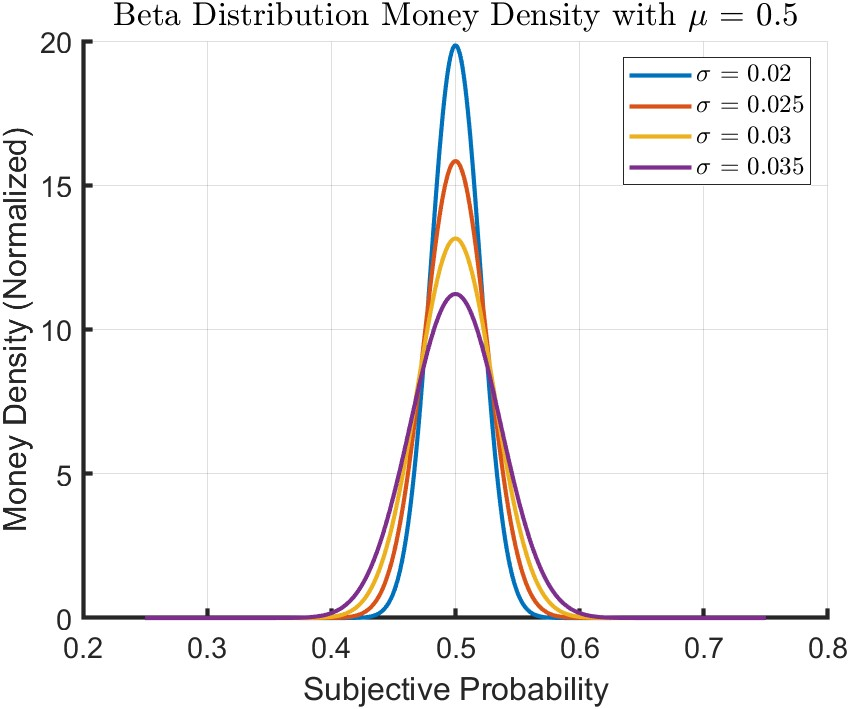
\includegraphics[width=8cm]{Beta Distribution}
	\caption{Modified Beta Distribution}
\end{figure}

I end this subsection with the hope that this paper inspires future research into subjective probability distributions. Specifically, research that queries subjective probabilities for outcomes across a variety of subjects and which attempts to mathematically model their distributions. 

\subsection{Comparing Synthesized Speculation and The Money Line}

This paper seeks to prove the dominance of the synthesized speculation system over the money line in two areas: user subjective expectation and sportsbook profit. These two metrics will be computed for each system over a set of subjective probability distributions. These subjective probability distributions will be modified beta distributions from the previous subsection, generated from a two dimensional mesh of $\mu$ and $\sigma$ values. Each distribution will be used to randomly generate 1000 subjective probability values, each with a corresponding bet amount randomly selected from a uniform distribution extending from $\$0$ to $\$100$. This configuration assumes the independence of subjective probability and bet amount, an assumption which can be altered in future research. The profit and user subjective expectation provided by each gambling system will then be computed. This will be done 30 times for each distribution to minimize the variability produced by randomly selection. These trials will inform 95$\%$ confidence intervals for user subjective expectation and sportsbook profit for both systems at each point in the $\mu \times \sigma$ mesh. The synthesized speculation system will be said to strictly dominate the traditional money line system for a given metric if, at each point in the $\mu \times \sigma$ mesh, the lower bound of the synthesized speculation confidence interval for that metric exceeds the upper bound of the corresponding money line confidence interval.

\subsection{Constructing The $\mu \times \sigma$ Mesh}

The $\mu$ mesh was informed by stipulations regarding subjective probability distributions for the intersection and union linakges of binary events, which is mathematically addressed in Appendix B. I first stipulate that the mean of the union of independent focal outcomes with equivalent means below the lowest mesh value must not exceed the maximum $\mu$ in the mesh. This is equivalent to the condition that the mean of the intersection of independent focal outcomes with equivalent means above the highest mesh value must not fall below the minimum $\mu$ in the mesh. These conditions ensure that, for an infinite set of focal outcomes with equivalent means $\mu > 0$, there must exist a finite subset of these outcomes that can be linked in such a way that the distribution mean falls with the $\mu$ mesh. Having solved for these conditions mathematically, I expanded the mesh range to align with more aesthetically pleasing values. Thus, the chosen $\mu$ mesh spans from .375 to .625, with .0625 spacing.

The $\sigma$ mesh, on the other hand, was generated using opening money line data from the 2023-24 NFL regular season, acquired from Action Network. Only money lines for which data was available (most games from weeks 6 to 18) and with $\frac{p_\alpha+p_\beta}{2}$ within the $\mu$ mesh were considered, the latter condition necessary to ensure that only distributions centered around the $\mu$ mesh informed the $\sigma$ mesh. Each opening money line was assumed to result from constrained optimization on a modified beta money density function, \a'a la subsection 1.3. Under this assumption, the $\mu$ and $\sigma$ of each money line's corresponding modified beta function were estimated using Monte Carlo sampling. For each money line, $\mu$ and $\sigma$ were chosen by selecting the sample $(\mu,\sigma)$ pair that minimized the maximum of the absolute value of Equations 11 and 12. Any ($\mu$, $\sigma$) pairs which did not regenerate the same money line when plugged into the modified beta money density function, within a margin of error of $\pm$2 for $\alpha$ and $\beta$, were eliminated from the data set. This left 73 NFL regular season games with $\sigma$ values derived through the assumption of a modified beta money density function and ideal constrained optimization by the sportsbook.

\begin{figure}[H]
	\centering
	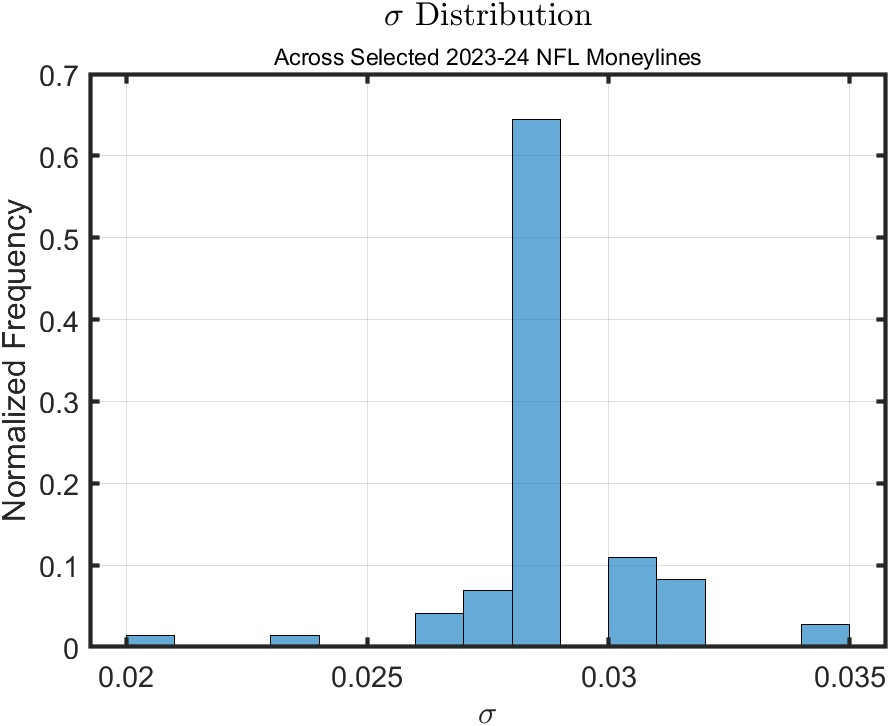
\includegraphics[width=11cm]{Selected NFL Sigma Distribution}
	\caption{$\sigma$ Distribution of Selected 2023-24 NFL Game Money Lines}
\end{figure}

The $\sigma$ values displayed above range from .021 to .034. As a validity check, a modified beta function with $\mu = .5$ and $\sigma = .03$ has a profit of roughly $4.2\%$ of the total money staked, close to the aforementioned standard of $4.5\%$. Using the data displayed in Figure 5, the $\sigma$ mesh spans from .02 to .035, with .005 spacing.

\section{Results}

\subsection{User Subjective Expectation}

Across the $\mu \times \sigma$ mesh, the synthesized speculation gambling system strictly dominated the traditional money line system with regard to user subjective expectation. The increase in mean user subjective expectation from the money line to the synthesized speculation system ranged from $32\%$ to $53\%$ across the mesh. The $95\%$ confidence intervals of user subjective expectation across the mesh are provided on the next page. 

% Subjective Expectation Results Table - Start
\newcolumntype{C}[1]{>{\centering\arraybackslash}m{#1}}
\renewcommand{\arraystretch}{3.8}
\setlength\extrarowheight{-.07cm}

\pagebreak
\begin{center}
	\begin{table}[ht]
	\centering
 	\textbf{\huge$\sigma$} \\
	\vspace{.05in}

	\begin{tabular}{ | C{2 cm} | C{2 cm} | C{2 cm} | C{2 cm} | C{2 cm}|}
	\hline
	                      & \large .02 & \large .025 & \large .03 & \large .035 \\
       \hline
	\large .375      & \begin{tabular}{@{}c@{}} $\textcolor{green}{[717,733]}$ \\ $\textcolor{red}{[492,544]}$ \end{tabular}
                              & \begin{tabular}{@{}c@{}} $\textcolor{green}{[898,911]}$ \\ $\textcolor{red}{[618,671]}$ \end{tabular}
                              & \begin{tabular}{@{}c@{}} $\textcolor{green}{[1076,1104]}$ \\ $\textcolor{red}{[780,843]}$ \end{tabular} 
                              & \begin{tabular}{@{}c@{}} $\textcolor{green}{[1257,1294]}$ \\ $\textcolor{red}{[872,938]}$ \end{tabular} \\
	\hline
	\large .4375    & \begin{tabular}{@{}c@{}} $\textcolor{green}{[747,762]}$ \\ $\textcolor{red}{[500,547]}$ \end{tabular} 
                              & \begin{tabular}{@{}c@{}} $\textcolor{green}{[935,954]}$ \\ $\textcolor{red}{[620,683]}$ \end{tabular}
                              & \begin{tabular}{@{}c@{}} $\textcolor{green}{[1101,1139]}$ \\ $\textcolor{red}{[710,788]}$ \end{tabular} 
                              & \begin{tabular}{@{}c@{}} $\textcolor{green}{[1285,1324]}$ \\ $\textcolor{red}{[894,960]}$ \end{tabular} \\	

	\hline
	\large .5          & \begin{tabular}{@{}c@{}} $\textcolor{green}{[756,777]}$ \\ $\textcolor{red}{[481,533]}$ \end{tabular} 
                              & \begin{tabular}{@{}c@{}} $\textcolor{green}{[947,962]}$ \\ $\textcolor{red}{[613,651]}$ \end{tabular} 
                              & \begin{tabular}{@{}c@{}} $\textcolor{green}{[1137,1164]}$ \\ $\textcolor{red}{[746,804]}$ \end{tabular} 
                              & \begin{tabular}{@{}c@{}} $\textcolor{green}{[1317,1350]}$ \\ $\textcolor{red}{[843,895]}$ \end{tabular} \\
        \hline
	\large .5625    & \begin{tabular}{@{}c@{}} $\textcolor{green}{[748,761]}$ \\ $\textcolor{red}{[518,558]}$ \end{tabular}
                             & \begin{tabular}{@{}c@{}} $\textcolor{green}{[919,942]}$ \\ $\textcolor{red}{[594,649]}$ \end{tabular}
                             & \begin{tabular}{@{}c@{}} $\textcolor{green}{[1107,1132]}$ \\ $\textcolor{red}{[757,822]}$ \end{tabular} 
                             & \begin{tabular}{@{}c@{}} $\textcolor{green}{[1286,1313]}$ \\ $\textcolor{red}{[880,939]}$ \end{tabular} \\
        \hline
	\large .625     & \begin{tabular}{@{}c@{}} $\textcolor{green}{[715,736]}$ \\ $\textcolor{red}{[507,560]}$ \end{tabular} 
                             & \begin{tabular}{@{}c@{}} $\textcolor{green}{[891,915]}$ \\ $\textcolor{red}{[626,678]}$ \end{tabular}
                             & \begin{tabular}{@{}c@{}} $\textcolor{green}{[1076,1106]}$ \\ $\textcolor{red}{[788,858]}$ \end{tabular} 
                             & \begin{tabular}{@{}c@{}} $\textcolor{green}{[1246,1274]}$ \\ $\textcolor{red}{[884,955]}$ \end{tabular} \\
        \hline
	\end{tabular}
    \begin{tablenotes}
        \item In each box, a \textcolor{green}{green} confidence interval strictly dominates a \textcolor{red}{red} confidence interval.
    \end{tablenotes}
	\caption{95$\%$ Confidence Intervals for Subjective Expectation}
	\end{table}
\end{center}
\vspace{-15pt}
%\pagebreak
% Synthesized Speculation and Money Line Labels
\begin{textblock*}{7cm}(17cm,4.5cm)\textbf{Synthesized} \end{textblock*} 
\begin{textblock*}{7cm}(17cm,5.5cm)\textbf{Money Line} \end{textblock*} 

\begin{textblock*}{7cm}(16.5cm,6.55cm)\textbf{Synthesized} \end{textblock*} 
\begin{textblock*}{7cm}(16.5cm,7.55cm)\textbf{Money Line} \end{textblock*} 

\begin{textblock*}{7cm}(16.5cm,8.6cm)\textbf{Synthesized} \end{textblock*} 
\begin{textblock*}{7cm}(16.5cm,9.6cm)\textbf{Money Line} \end{textblock*} 

\begin{textblock*}{7cm}(16.5cm,10.65cm)\textbf{Synthesized} \end{textblock*} 
\begin{textblock*}{7cm}(16.5cm,11.65cm)\textbf{Money Line} \end{textblock*} 

\begin{textblock*}{7cm}(16.5cm,12.65cm)\textbf{Synthesized} \end{textblock*} 
\begin{textblock*}{7cm}(16.5cm,13.65cm)\textbf{Money Line} \end{textblock*} 
% Side Axes Label Must be Adjusted Along With Other Adjustements to Previous Sections
\begin{textblock*}{7cm}(3.25cm,9cm) \rotatebox[origin=c]{90}{\textbf{\huge$\mu$}} \end{textblock*}

However, the increase in subjective expectation was not uniform across the user base. To demonstrate this, the subjective expectation value of each player was computed as a function of subjective probability for a trial at the $\mu = .625$, $\sigma = .03$ mesh point. This subjective probability distribution had the lowest increase in average user subjective expectation and was chosen to minimize any bias toward the synthesized speculation system.  For this example, the bet amounts were set to $\$7.5$ to ensure a reasonable blend of peer and money line bets. The consequent plot of subjective expectation vs subjective probability follows.

\begin{figure}[H]
	\centering
	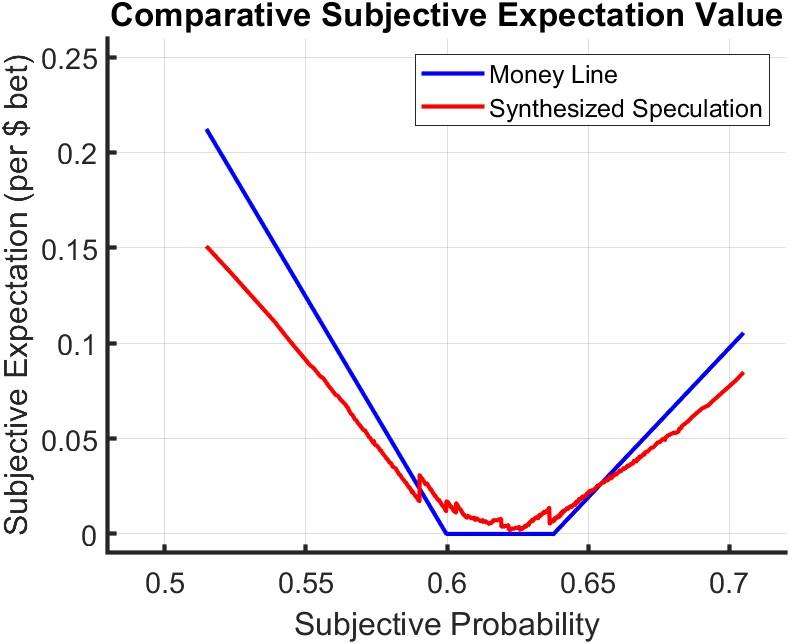
\includegraphics[width=10cm]{Subjective Expectation Comparison}
	\caption{Subjective Expectation Across User Base}
\end{figure}

As Figure 6 shows, the synthesized speculation system provides users with subjective probabilities close to the median a higher subjective expectation than the money line system. Only at more extreme subjective probabilities does the money line system offer more subjective expectation. In this case, the thresholds at which the optimal gambling system for subjective expecation changes is $p = .59$ and $p = .65$. The accumulated money density within this interval corresponds to approximately $66\%$ of all bet amounts. 

\subsection{Sportsbook Profit}

Across the $\mu \times \sigma$ mesh, the synthesized speculation gambling system strictly dominated the traditional money line system in terms of sportsbook profit. The increase in mean sportsbook profit from the money line to the synthesized speculation system ranged from $6\%$ to $17.4\%$ across the mesh. The $95\%$ confidence intervals of sportsbook profit across the mesh are provided on the subsequent page. 

% Profit Results Table - Start
\newcolumntype{C}[1]{>{\centering\arraybackslash}m{#1}}
\renewcommand{\arraystretch}{3.8}
\setlength\extrarowheight{-.07cm}

\pagebreak
\begin{center} 
	\begin{table}[ht]
	\centering
 	\textbf{\huge$\sigma$} \\
	\vspace{.05in}

	\begin{tabular}{ | C{2 cm} | C{2 cm} | C{2 cm} | C{2 cm} | C{2 cm}|}
	\hline
	                      & \large .02 & \large .025 & \large .03 & \large .035 \\
       \hline
	\large .375      & \begin{tabular}{@{}c@{}} $\textcolor{green}{[737,754]}$ \\ $\textcolor{red}{[687,707]}$ \end{tabular}
                              & \begin{tabular}{@{}c@{}} $\textcolor{green}{[924,946]}$ \\ $\textcolor{red}{[846,870]}$ \end{tabular}
                              & \begin{tabular}{@{}c@{}} $\textcolor{green}{[1101,1136]}$ \\ $\textcolor{red}{[1017,1048]}$ \end{tabular} 
                              & \begin{tabular}{@{}c@{}} $\textcolor{green}{[1270,1305]}$ \\ $\textcolor{red}{[1195,1234]}$ \end{tabular} \\
	\hline
	\large .4375    & \begin{tabular}{@{}c@{}} $\textcolor{green}{[748,767]}$ \\ $\textcolor{red}{[668,688]}$ \end{tabular} 
                              & \begin{tabular}{@{}c@{}} $\textcolor{green}{[935,952]}$ \\ $\textcolor{red}{[833,854]}$ \end{tabular}
                              & \begin{tabular}{@{}c@{}} $\textcolor{green}{[1098,1134]}$ \\ $\textcolor{red}{[990,1026]}$ \end{tabular} 
                              & \begin{tabular}{@{}c@{}} $\textcolor{green}{[1297,1327]}$ \\ $\textcolor{red}{[1163,1193]}$ \end{tabular} \\	

	\hline
	\large .5          & \begin{tabular}{@{}c@{}} $\textcolor{green}{[768,789]}$ \\ $\textcolor{red}{[653,674]}$ \end{tabular} 
                              & \begin{tabular}{@{}c@{}} $\textcolor{green}{[964,978]}$ \\ $\textcolor{red}{[818,836]}$ \end{tabular} 
                              & \begin{tabular}{@{}c@{}} $\textcolor{green}{[1158,1183]}$ \\ $\textcolor{red}{[990,1015]}$ \end{tabular} 
                              & \begin{tabular}{@{}c@{}} $\textcolor{green}{[1336,1371]}$ \\ $\textcolor{red}{[1136,1169]}$ \end{tabular} \\
        \hline
	\large .5625    & \begin{tabular}{@{}c@{}} $\textcolor{green}{[749,761]}$ \\ $\textcolor{red}{[670,687]}$ \end{tabular}
                             & \begin{tabular}{@{}c@{}} $\textcolor{green}{[925,946]}$ \\ $\textcolor{red}{[820,841]}$ \end{tabular}
                             & \begin{tabular}{@{}c@{}} $\textcolor{green}{[1105,1131]}$ \\ $\textcolor{red}{[987,1018]}$ \end{tabular} 
                             & \begin{tabular}{@{}c@{}} $\textcolor{green}{[1295,1318]}$ \\ $\textcolor{red}{[1166,1193]}$ \end{tabular} \\
        \hline
	\large .625     & \begin{tabular}{@{}c@{}} $\textcolor{green}{[741,762]}$ \\ $\textcolor{red}{[682,703]}$ \end{tabular} 
                             & \begin{tabular}{@{}c@{}} $\textcolor{green}{[912,934]}$ \\ $\textcolor{red}{[839,864]}$ \end{tabular}
                             & \begin{tabular}{@{}c@{}} $\textcolor{green}{[1100,1135]}$ \\ $\textcolor{red}{[1022,1054]}$ \end{tabular} 
                             & \begin{tabular}{@{}c@{}} $\textcolor{green}{[1288,1310]}$ \\ $\textcolor{red}{[1178,1218]}$ \end{tabular} \\
        \hline
	\end{tabular}
    \begin{tablenotes}
        \item In each box, a \textcolor{green}{green} confidence interval strictly dominates a \textcolor{red}{red} confidence interval.
    \end{tablenotes}
	\caption{95$\%$ Confidence Intervals for Profit}
	\end{table}
\end{center}
\vspace{-15pt}
%\pagebreak
% Synthesized Speculation and Money Line Labels
\begin{textblock*}{7cm}(17cm,4.5cm)\textbf{Synthesized} \end{textblock*} 
\begin{textblock*}{7cm}(17cm,5.5cm)\textbf{Money Line} \end{textblock*} 

\begin{textblock*}{7cm}(16.5cm,6.55cm)\textbf{Synthesized} \end{textblock*} 
\begin{textblock*}{7cm}(16.5cm,7.55cm)\textbf{Money Line} \end{textblock*} 

\begin{textblock*}{7cm}(16.5cm,8.6cm)\textbf{Synthesized} \end{textblock*} 
\begin{textblock*}{7cm}(16.5cm,9.6cm)\textbf{Money Line} \end{textblock*} 

\begin{textblock*}{7cm}(16.5cm,10.65cm)\textbf{Synthesized} \end{textblock*} 
\begin{textblock*}{7cm}(16.5cm,11.65cm)\textbf{Money Line} \end{textblock*} 

\begin{textblock*}{7cm}(16.5cm,12.65cm)\textbf{Synthesized} \end{textblock*} 
\begin{textblock*}{7cm}(16.5cm,13.65cm)\textbf{Money Line} \end{textblock*} 
% Side Axes Label Must be Adjusted Along With Other Adjustements to Previous Sections
\begin{textblock*}{7cm}(3.25cm,9cm) \rotatebox[origin=c]{90}{\textbf{\huge$\mu$}} \end{textblock*}

To better illustrate the enhanced performance of the synthesized speculation system, Figure 7 displays a contour plot of the percent change in average sportsbook profit from the money line to the synthesized speculation system. The contour plot is interpolated across the $\mu \times \sigma$ mesh using the data from Table 4. 

\begin{figure}[H]
	\centering
	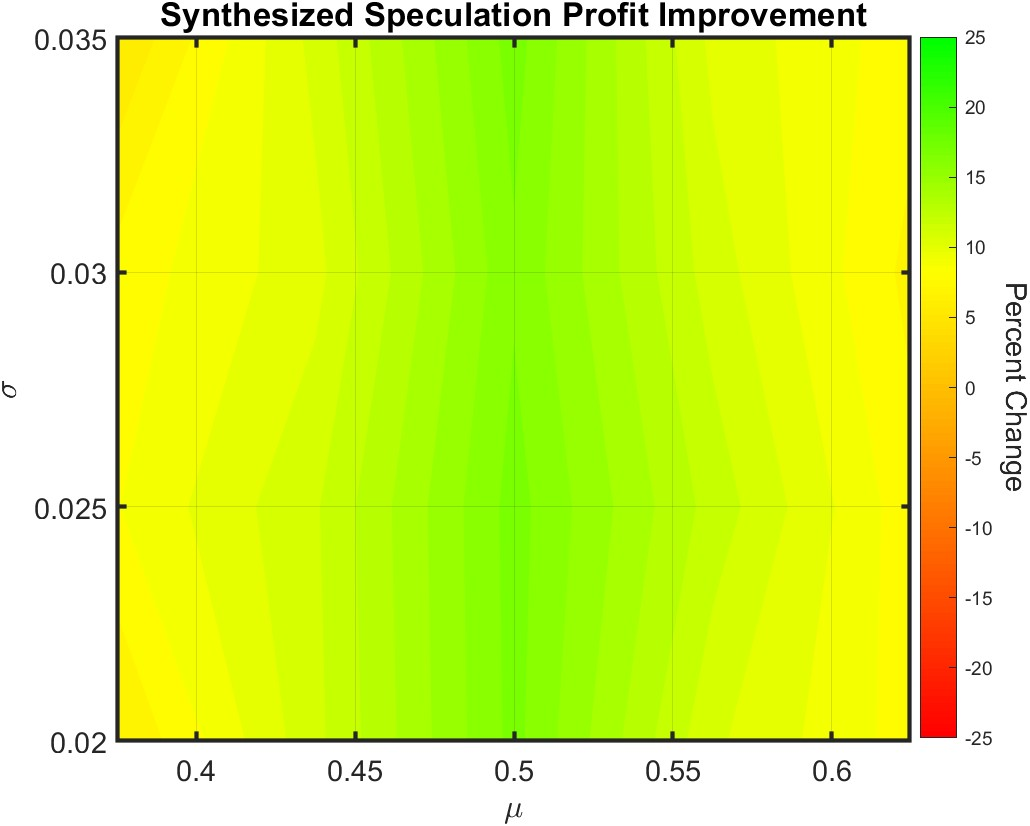
\includegraphics[width=10cm]{Profit Contour}
	\caption{Profit Improvement from Money Line to Synthesized Speculation}
\end{figure}

This plot makes clear that the maximum profit increase occurs along the line $\mu = .5$, where it reaches a maximum of $17.4\%$. As $\mu$ diverges from $.5$ to the bounds of the $\mu$ mesh, the growth in sportsbook profit from the money line to synthesized speculation declines considerably. However, even at the edges of the mesh, this growth never dips below $5\%$. 

\section{Discussion}

\subsection{Explaining Synthesized Speculation Dominance}

The natural response to the dominance of the synthesized speculation system in both user subjective expectation and sportsbook profit is skepticism. The key distinction here is the difference between user subjective expectation and actual user returns. The synthesized speculation system is designed to reward informed speculation. Customers with knowledgeable subjective probabilities will likely produce profit in the long run. Customers with misinformed and ill researched subjective probabilities will likely lose money over time. This is simply the synthesized speculation manifestation of the sharp vs. square gambling dynamic common in money lines. What differentiates the synthesized speculation system is that it allows informed bettors to get more positive expectation, often at lower risk. This is evident across the paper, from Table 3 to Figure 6 to Figure 12 in Appendix C. 

The synthesized speculation system can have sizeable payouts while maintaining profit dominance because it engages a larger share of customer money in bets. Under the assumption of static subjective probabilities, users in the subjective probability no man's land of $p_\beta < p < p_\alpha$ have no positive subjective expectation bets available in a money line. As such, they place no bets with the monye line and their money remains unemployed. Across the $\mu \times \sigma$ mesh, this consequently left a massive amount of money on the table, ranging from $43\%$ to $58\%$ of the total bet money available. In comparison, the synthesized speculation system only failed to utilize $.3\%$ to $6.3\%$ of bet amounts, mainly from slice straddles and the small no man's land of the iterative money line. The slice straddles occurred when players with large bet amounts and moderate subjective probabilities had peer bet slices that straddled the median subjective probability, leading to the player being assigned to bet against themselves. The synthesized speculation system currently considers these slices as wasted money, but further models could incorporate this money into the iterative money line. 

As a final note, the ratio of sportsbook profit to user subjective expectation can be manipulated via the $\lambda$ parameter. This ratio is roughly equivalent to $\frac{\lambda}{2}$, as $\lambda$ is the ratio of sportsbook profit to a single slice's subjective expectation value in a peer bet. To boost sportsbook profit, $\lambda$ may be increased, though user subjective expectation decreases to zero as $\lambda$ approaches infinity. 

\subsection{Optimal Synthesized Speculation Use Cases}

As Figure 7 demonstrates, the profit improvement from the money line to the synthesized speculation system is most profound around $\mu = 0.5$. This likely arises from the increase in total peer bet stakes as the subjective probability distribution becomes clustered around 0.5. Indeed, a subjective probability distribution symmetric about a mean of 0.5 will fully engage each slice's bet amount, as evident from the use case  $p_< + p_> = 1$ in Table 2. Though dependent on $\lambda$, customers stakes are generally more profitably placed in peer bets rather than the iterative money line. Thus, the synthesized speculation system is recommended for use with subjective probability distributions centered around half unity. 

Furthermore, the synthesized speculation system is ideal for binary events for which a money line does not exist. The reasoning is that, as illustrated in Figure 6, customers with extreme subjective profitabilities have higher subjective expectation with the money line, and will likely defect. This will eliminate the most profitable subset of customers, as the $\lambda$ convention of peer bet stake assignment ensures that sportsbook profit is roughly proportional to user subjective expectation within peer bets. Finally, the synthesized speculation system is superior for use for binary events without pre-existing money lines, as it does not require the service of professional oddsmakers to assign betting odds. Instead, oddsmaking is democritized in such a manner as to reward informed speculation. Binary events, such as innovative parlays of semi-coupled constituent binary events, could be created to offer these unique betting opportunities.

In light of these qualities, this paper recommends the synthesized speculation system as a supplement to the money line rather than a replacement. Unions and intersections can be used to link binary outcomes in such a manner as to encourage a subjective probability distribution centered around half unity and create a unique focal outcome outside the traditional scope of money lines. The synthesized speculation system could be advertised as a way for customers to be their own oddsmaker, researching and speculating in order to outperform their peers. According to academic research, $65\%$ of Americans believe that they are smarter than the average person (Heck et. al, 2018). The synthesized speculation system gives them a chance to prove it. With this system, sportsbook vigorish is not an upfront barrier to entry for customers with moderate subjective probabilities; it is an incentive for the sportsbook to provide positive subjective expectation bets. 

\subsection{Next Steps}

This paper is intended to stimulate interest in alternative betting systems to the money line. As stated earlier, the synthesized speculation system is not the only nor necessarily the most profitable configuration that can be made using the subsystems described. While the numerical comparison with the money line was informative, a statistical analysis is only as accurate as the data which underpins it. I recommend further research into the distribution of subjective probability, looking at a wide variety of binary events as the Andersen et. al paper did. The binary events in question could even include unions and intersections of constituent binary events, especially interdependent ones. Questions also remain regarding the dependence of betting amount on subjective probability. 

In additional to more fundamental questions, technical questions also exist. For my results in Section 5, I randomly generated user subjective probability without specify a minimum probability increment. This resulted in probability spacings as low as one in ten million. Since the synthesized speculation system benefits from betting asymmetry, implementing a finite probability spacing may limit profitability or, in the case of favorable rounding, increase it. This bears looking into, as does whether the optimal slice amount is $\$5$.

Ultimately, the most effective method to learn more about the synthesized speculation system would be to implement it. This would provide real time access to subjective probability and bet distributions, as well as various arbitrage strategies. Submitted subjective probabilities may not reflect customer beliefs expressed in academic surveys, as users adjust their probabilities to manipulate the system (see Appendix C). Comparison between customer surveys and actual submissions would help answer questions regarding this effect. While simple arbitrage strategies are discussed in Appendix D, more complex strategies may exist and would be exposed with the system's execution. However, in addition to the standard challenges of funding and website design, implementing the synthesized speculation system would require new legistlation at the state level. That said, the recent success of sports gambling and betting exchange legislation provide grounds for optimism. I believe that the benefits of the synthesized speculation system would be well worth the effort of realization. As shown by my analysis, the synthesized speculation system has the potential to better reward informed speculation while boosting sportsbook profit. I hope that, one day, it is given a chance to prove it.

\pagebreak 

\appendix
\section{Matching Strategies}

The set of unique matches among $N$ players (with $N$ even) can be generated recusively from the set of unique matches among $N-2$ players. This recursion algorithm first generates all of the possible matches between the first player and the remaining $N-1$ players. For each of these matches, the residual $N-2$ players are matched according to the $N-2$ unique matching strategies. This is accomplished by utilizing the player numbers of the $N-2$ unique matching strategy as indeces for the remaining player numbers. For example, the $1$ in the $N-2$ matching strategy would correspond to the lowest remaining player number, $2$ would correspond to the second lowest, et cetera. The generation of unique matches among $N = 6$ players from the set of unique matches among $N = 4$ players is shown below in Figure 8.

\begin{figure}[H]
	\centering
	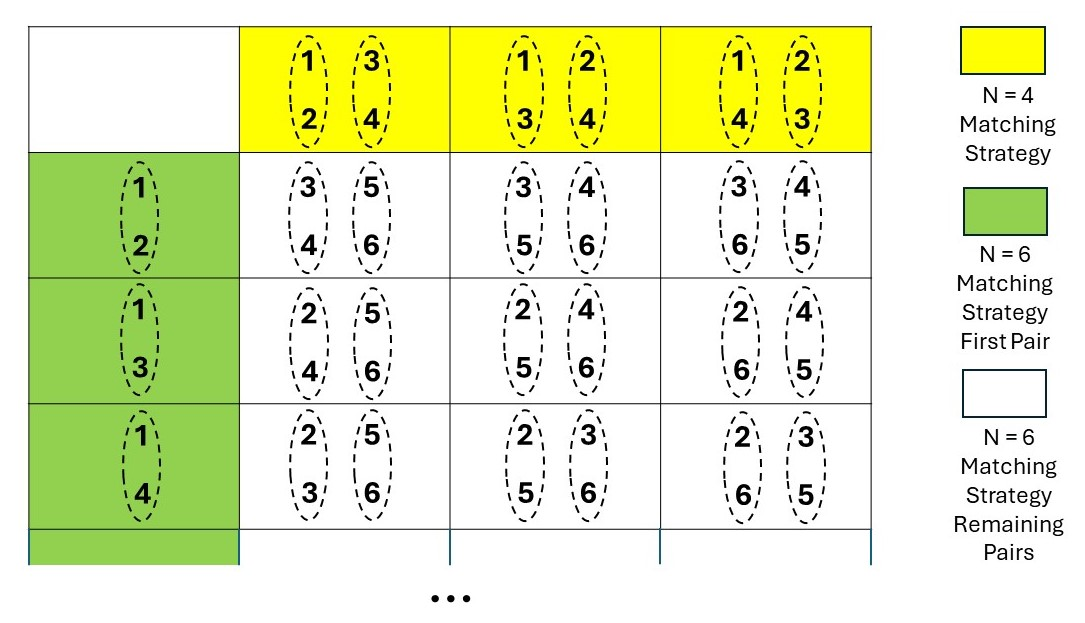
\includegraphics[width=12cm]{Iterative Matching Generation}
	\caption{Generating Unique Matching Strategies Recursively}
\end{figure}

Thus, the number of unique matches among $N$ players is equal to $N-1$ times the number of unique matches among $N-2$ players. 
Given this recursive relation and that the number of unique matches among two players is one, the number of unique matches among $N$ players (defined as $M(N$)) must equal the following:

\begin{equation}
M(N) = \frac{N!}{2^{N/2}(\frac{N}{2})!}
\end{equation}
\vspace{.05in}

As evident above, $M(N)$ grows factorially with $N$. At $N = 10$, there are 945 unique matching stratgies. As $N$ grows to 16, the number of unique matches exceeds two million and once $N$ equals 100, the number of unique matches is on the order of $10^{78}$. Thus, as $N$ increases, evaluating the profitability of each unique match quickly stresses compuational resources. Ideally, there would exist a simple matching strategy that offers a high level of profitability relative to the other matching strategies. To prove the existence of such a strategy, the profit from simple matching strategy of outside-in matching (described in subsection 3.5) was compared to all of the possible matching strategies for a sample of $N = 16$ slices from a uniform subjective probability distrubution across $[0, 1]$. 

The profit of each matching strategy was averaged across 100 trials. In each trial, profit was computed by implementing a peer to peer bet for each pairing, and summing the rake from each bet. Within each bet, $\lambda$ was set equal to $2$, with a slice size equal to \$1. The results are shown below in Figure 9.

\begin{figure}[H]
	\centering
	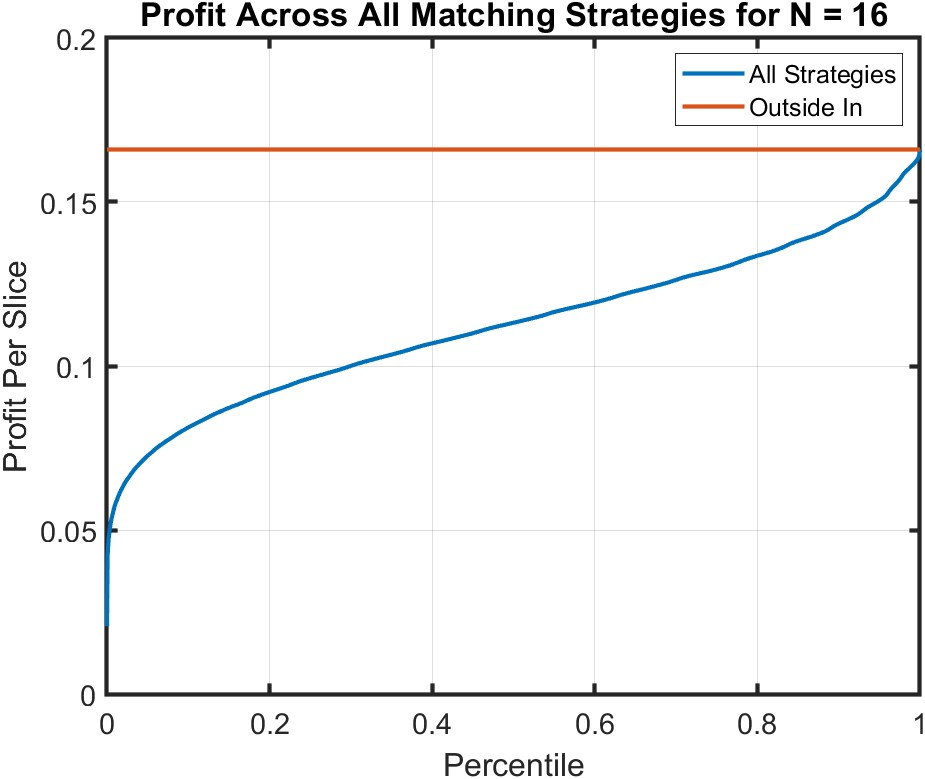
\includegraphics[width=10cm]{Matching Strategy Profit}
	\caption{Average Profit per Slice with Different Matching Strategies}
\end{figure}

As shown above, the outside-in strategy has an average profit across the 100 trials that outperforms a vast majority of the other strategies. Of the 2,027,025 unique matching strategies for $N =16$, only 14 strategies had a higher average profitability across the 100 trials. The strategies that did outperform outside-in  did so marginally, with the best at an average profit of $\$.1661$ per dollar bet compared to $\$.1660$ for outside-in. That said, Figure 9 addresses the average profitability across trials, not the indiviudal trials themselves. To compare outside-in to the other matching strategies across each trial, please reference Figure 10 on the succeeding page. 

\begin{figure}[H]
	\centering
	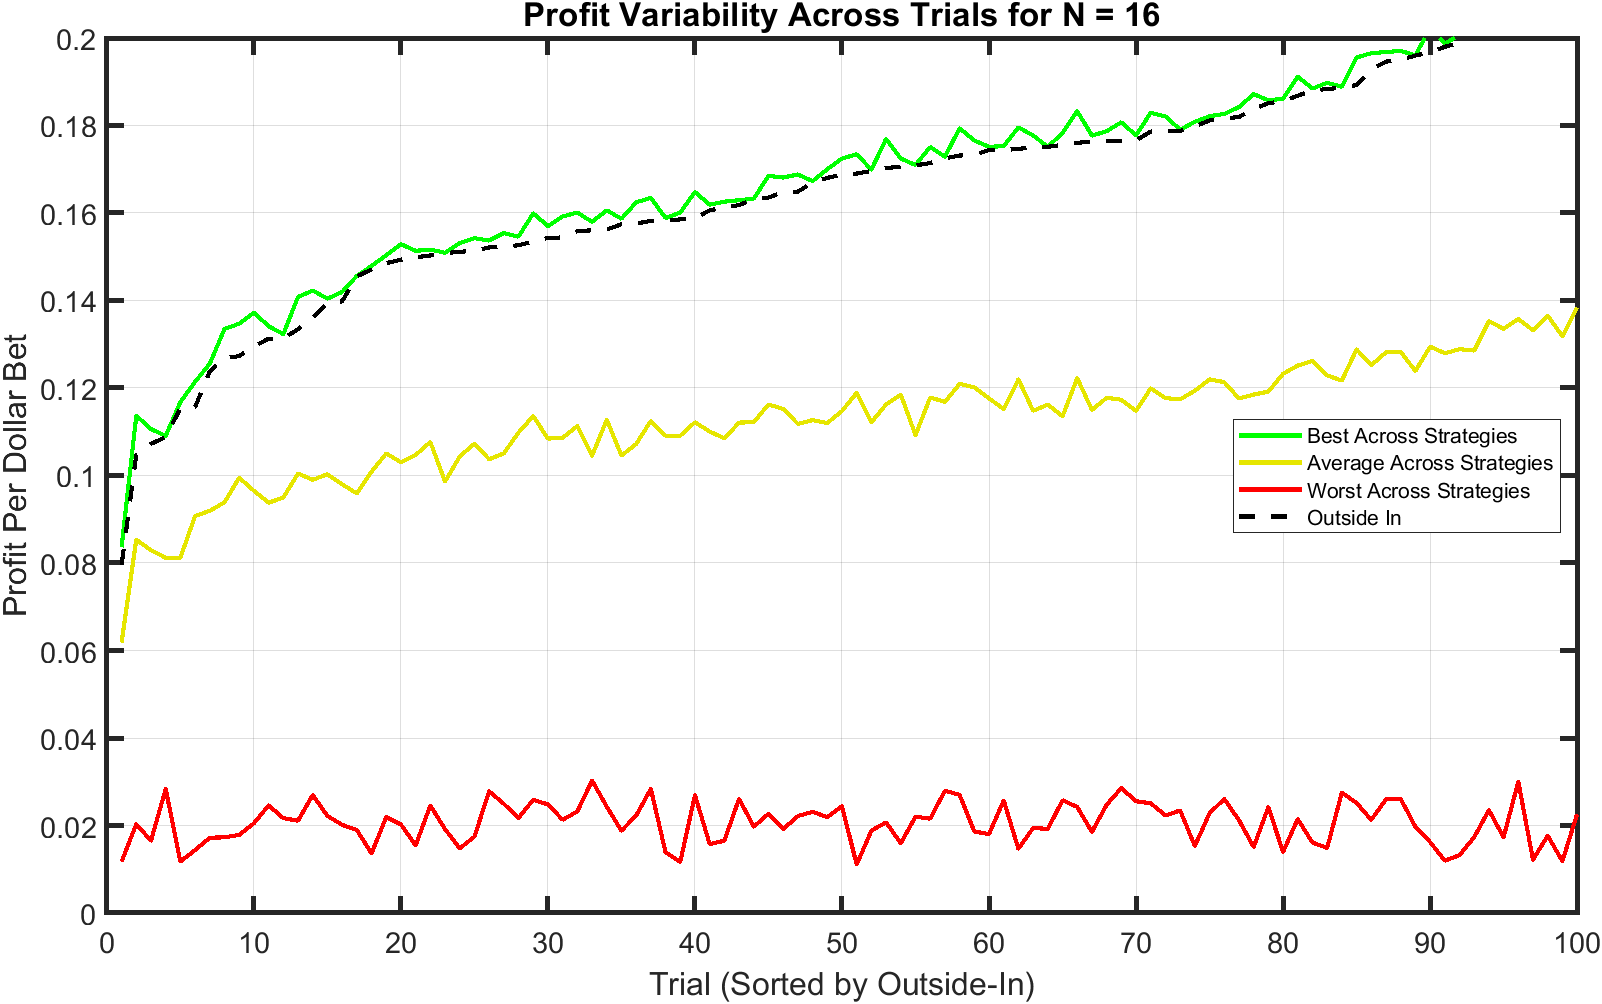
\includegraphics[width=13cm]{Matching Strategy Outcomes Across Trials}
	\caption{Matching Strategy Outcomes Across Trials}
\end{figure}

Again, the outside-in strategy has a high degree of profitability relative to the other matching strategies, falling only marginally below the best strategy in each trial. Given the simplicity of the outside-in matching system, and its high level of profitability, I recommend it as a matching strategy for peer bets within the synthesized speculation system.

\section{Combining Multiple Binary Events}

\subsection{Overview}

As evident across Tables 3 and 4, higher variability within the money density function increases user subjective expectation and sportsbook profit. As typical in commerical markets, greater value asymmetry increases the profit margins of market makers and allows customers more opportunity for what they perceive as good deals. Money density function variation may be increased by the union and intersection of binary event outcomes. Intersections would define the focal outcome as the occurence of both constituent outcomes. In constrast, unions would link two outcomes by defining the focal outcome as the occurence of at least one of the these constituent outcomes. The effects of both intersection and union linkages between two subjective probability distributions $\rho_X$ and $\rho_Y$ (with the resulting probability distibution labelled $\rho_Z$) will be examined in the following subsections. In addition to boosting variation, these linkages can shift the money density mean closer to the ideal of half unity. These results can be mapped to money density distributions with the assumption that betting amount is independent of subjective probability and that the subjective probabilities for the binary events are independent of each other. For the sake of thoroughness, the effect of linkages on dependent random variables will also be included. 

% AND
\subsection{Intersection of Outcomes}

\begin{equation}
z = x y
\end{equation}
\vspace{.05in}

Given that a subjective probability for focal outcome one is distributed as $\rho_X$, the subjective probability for focal outcome two is distributed as $\rho_Y$, and that these subjective probabilities are independent, we can compute the distribution for the subjective probability that both focal outcomes occur. This is simply the distribution for the product of the subjective probabilities from $\rho_X$ and the ones from $\rho_Y$. As such, we can use the standard formula for the distribution of product of random variables, which will be denoted $\rho_Z$ (Rohatgi and Saleh, 2001).

\begin{equation}
\rho_Z(z) = \int_{0}^{1}\rho_X(x) \rho_Y(\frac{z}{x})\frac{1}{x}dx
\end{equation}
\vspace{.05in}

The corresponding mean and variance of $\rho_Z$, denoted $\mu_Z$ and $\sigma_Z$ respectively, are the following (Goodman, 1960):

\begin{equation}
\mu_Z = \mu_X \mu_Y
\end{equation}

\begin{equation}
\sigma_Z^2 = \sigma_X^2 \sigma_Y^2 + \mu_X^2 \sigma_Y^2 + \mu_Y^2 \sigma_X^2
\end{equation}
\vspace{.05in}

Ideally, $\mu_Z$ would be approximate to $\frac{1}{2}$, as subjective probability distributions with means closer to half unity had higher user subjective expectation and sportsbook profit across the $\mu \times \sigma$ mesh. Higher $\mu_X$ and $\mu_Y$ also increase $\sigma_Z$, which should exceed both $\sigma_X$ and $\sigma_Y$. Otherwise, our focal outcome would ideally be the focal outcome of $\rho_X$ or $\rho_Y$, depending on which had higher variability. If $\rho_X$ and $\rho_Y$ are identical distributions, $\mu = \frac{1}{\sqrt{2}}$ guarantees that $\sigma_Z > \sigma_X$. Therefore, intersection linkages are recommend for linking two focal outcomes with subjective probability distributions centered above $\frac{1}{\sqrt{2}} \approx .707$, which would individually have lower potential for user subjective expectation and sportsbook profit than a subjective probability distribition for the intersection of these two outcomes. 

% OR
\subsection{Union of Outcomes}

\begin{equation}
z = x + y - x y
\end{equation}
\vspace{.05in}

As in the case of intersection, the subjective probability distribution for the union of two focal outcomes can be computed under the assumption of independence between the subjective probability distributions of both focal outcomes. The distribution formula is similar to that of intersection, with the argument of $\rho_Y$ expressed as function of $x$ and $z$ using Equation (22). The integrand is multiplied by the derivative of this function with respect to $z$ to correct the differential element.

\begin{equation}
\rho_Z(z) = \int_{0}^{1}\rho_X(x) \rho_Y(\frac{z-x}{1-x})\frac{1}{1-x}dx
\end{equation}
\vspace{.05in}

The mean and variance of this new $\rho_Z$ are as follows:

\begin{equation}
\mu_Z = \mu_X + \mu_Y - \mu_X \mu_Y
\end{equation}

\begin{equation}
\sigma_Z^2 = \sigma_X^2 \sigma_Y^2 + (1-\mu_X)^2 \sigma_Y^2 + ( 1-\mu_Y)^2 \sigma_X^2
\end{equation}
\vspace{.05in}

The formula for the standard deviation is derived using Equation 21. Since the union outcome doesn't occur only if both focal outcomes don't occur, the union linkage has the same variability as an intersection between the corresponding compliment outcomes. Thus, the $\mu_X$ and $\mu_Y$ of Equation (21) are replaced with $1-\mu_X$ and $1-\mu_Y$. In the case where $\rho_X$ and $\rho_Y$ are identical distributuons, $\mu = 1-\frac{1}{\sqrt{2}}$ guarantees that $\sigma_Z > \sigma_X$. Therefore, union linkages are recommend for linking two focal outcomes with subjective probability distributions centered around $1-\frac{1}{\sqrt{2}} \approx .293$, which would individually have lower potential for user subjective expectation and sportsbook profit than a subjective probability distribition for the union of these two outcomes. 

\subsection{Dependent Random Variables}

For thoroughness, the mean and variance for the intersection and union of dependent binary outcomes are also included. As in the case of independent binary  event outcomes, there exist some correlated distributions for which an intersection or union linkage may result in a distribution with a mean closer to half unity and increased variation. Given the additional complexity of dependence, finding such distributions may not be as straightforward. Computing the resulting mean and variance for dependent variables now requires the computation of covariances in addition to the individual means and variances. The formulas for computing the mean and variance of $\rho_Z$, where $z = x y$ is the intersection of random variables $X$ and $Y$, is below:

\begin{equation}
\mu_Z = \mu_X \mu_Y + cov(X,Y)
\end{equation}

\begin{equation}
\sigma_Z^2 = \sigma_X^2 \sigma_Y^2 + \mu_X^2 \sigma_Y^2 + \mu_Y^2 \sigma_X^2 + cov(X^2,Y^2) - cov(X,Y)^2 - 2  \mu_X \mu_Y cov(X,Y)
\end{equation}
\vspace{.05in}

The mean and variance of $\rho_Z$, where  $z = x + y - x y$ is the union of random variables $X$ and $Y$, follows:

\begin{equation}
\mu_Z = \mu_X + \mu_Y - \mu_X \mu_Y - cov(X,Y)
\end{equation}

\begin{dmath}
\sigma_Z^2 = \sigma_X^2 \sigma_Y^2 + (1-\mu_X)^2 \sigma_Y^2 +
+ (1-\mu_Y)^2 \sigma_X^2 + cov((1-X)^2,(1-Y)^2) \hspace{.4in} - cov(X,Y)^2 - 2 (1-\mu_X)(1-\mu_Y) cov(X,Y) \hspace{1in}
\end{dmath}
\vspace{.05in}

In the event that all covariances are set to zero, the equations of subsection B.4 regress to the equations of subsections B.2 and B.3. 

\section{Gaming the System}

Within the synthesized speculation gambling system, user subjective expectation is not necessarily maximized with an accurate subjective probability. In the terms of probability assessment, the synthesized speculation reward structure is not a strictly proper scoring rule in the manner of the Brier score (Bickel, 2007). Instead, users can enhance their subjective expectation by inflating or depressing their subjective probability upon submission. However, over-adjustments can result in the assignment of the wrong win condition, necessitating a degree of finesse. In the correct application, users can adjust their subjective probability and bet amount to select the optimal (risk,reward) option, in a manner akin to Markowitz's portfolio selection (1952).

To exemplify this process, consider a money density function in the form of a modified beta distribution with parameters $\mu = .55$, $\sigma = .03$. The median is almost identical to the mean, at .5505. I assume that the user knows this, along with the true focal outcome probability of .5. To generate a set of (risk, reward) options, 1000 subjective probabilities were randomly selected from this $\rho_M$ and assigned a random bet amount from a uniform distribution across the domain $[\$10, \$100]$. Their probabilities and bet amounts were assigned bets using the synthesized speculation system. The expected value and standard deviation per dollar bet, determined using the true focal probability of .5, was computted for each player. These pairs are plotted in Figure 11, with their iterative money line position indicated by color.

\begin{figure}[H]
	\centering
	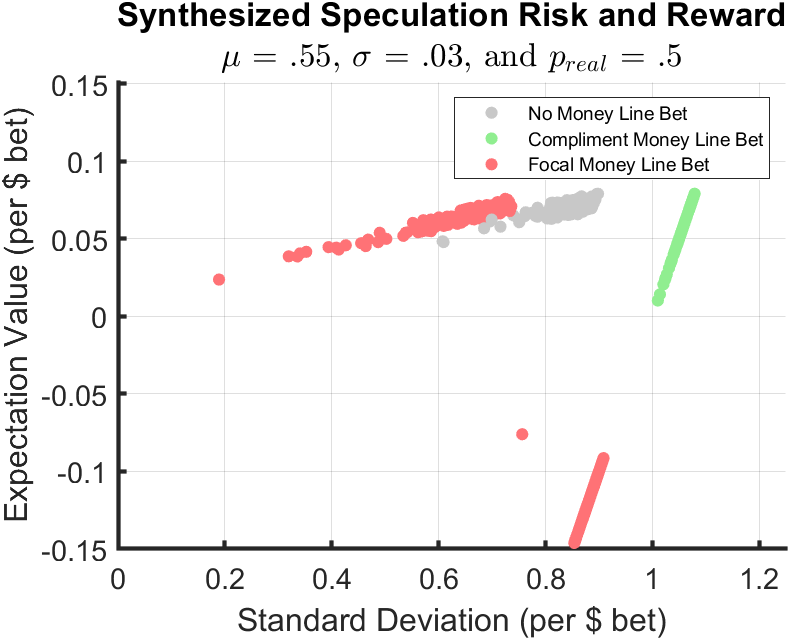
\includegraphics[width=10cm]{E_vs_V_Categories}
	\caption{Risk and Reward by Money Line Position}
\end{figure}

Using bet standard deviation as a proxy for risk and expectation value as one for reward, Figure 11 reveals that the synthesized speculation system offers an expansive set of (risk,reward) options. The effect of the iterative money line position on these options was profound. Players with iterative money line bets on the focal outcome had negative expectation if their subjective probability exceeded the median, as both their peer and money line bets were on a focal outcome whose payouts were undervalued according to the real focal probability. While players with money line bets on the compliment outcome and with no money line bets at all tended to have positive expectation, these player still maintained high values of risk. The ideal (risk,reward) subspace occurred when players had subjective probabilities below the median and money line bets on the focal outcome. In this subspace, players reduced risk by leveraging their peer bet on the compliment outcome against their money line bet on the focal outcome. Since $p_\alpha$ was less than the true focal probability, money line bets on the focal outcome added expectation as the money line overcompensated players for this bet. Figure 12 looks at this ideal subspace in greater detail. 

\begin{figure}[H]
	\centering
	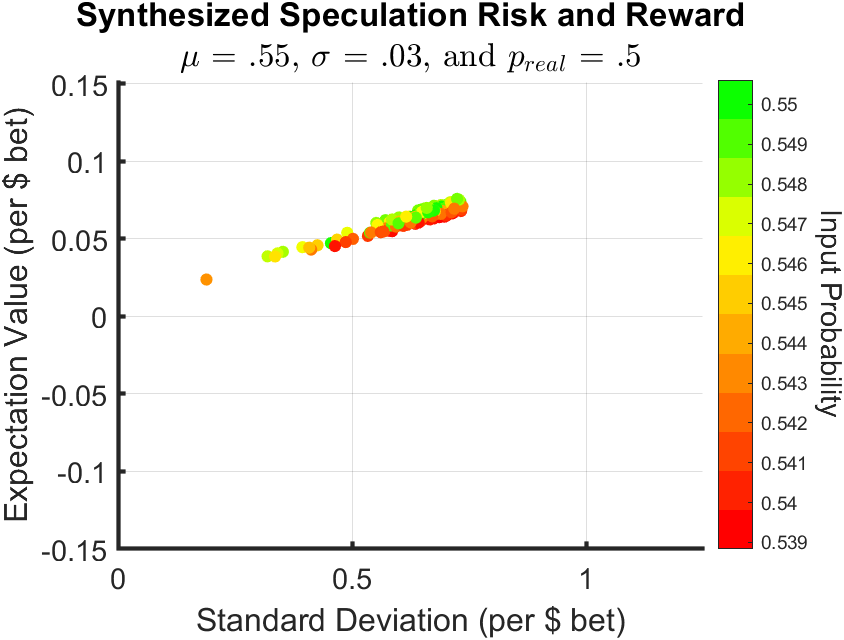
\includegraphics[width=10cm]{E_vs_V_Individual}
	\caption{Risk and Reward for Subset of Input Probabilities}
\end{figure}

Across the (risk,reward) space in Figure 12, a rise in risk corresponds with a rise in reward. This aligns with the concept of a risk premium in financial mathematics, where investments with higher risk compensate by offering a higher return. Users may move along this line by adjusting the residual money left over from bet slicing. For slice amounts of $\$5$, the residual money from bet slicing can be boosted by increasing the bet amount modulo five. This option reduces reward by decreasing the percent of money staked in peer bets, which have better payoff ratios in this subspace for this example. However, it also it reduces risk by hedging more money against the existing peer bet.

The submitted probability determines the slope of the risk vs reward line. In this case, the closer a user's submitted probability is to the median (without exceeding it), the higher the slope is. The left skew of $\rho_M$ ensures that $p_< + p_>$ is maximized for outside-in matches with percentiles closer to the median, boosting the payout ratios for the compliment position of those peer bets. This boosted payout ratio, in turn, increases the differential in risk and reward as a marginal dollar is transferred from the iterative money line to the peer bet. 

I will finish this subsection by noting that while the synthesized speculation system offers an expansive array of (risk,reward) options, the traditional money line only offers three. The first option is trivial, the option to bet nothing. The second option is to bet on the focal outcome, which, because the median subjective probability significantly exceeds the true focal probability in this example, has negative expectation value. The only viable option remaining, betting on the compliment outcome, has a standard deviation of $\$$1.05 and an expected value of $\$$.05 per dollar bet. As you can see in Figure 12, this option has both elevated risk and diminished returns relative to a number of synthesized speculation options, making the option set for the traditional money line objectively worse in this given example.

\section{Arbitrage}

\subsection{Introduction}

The search for arbitrage opportunities is an essential feature of any financial market, and acts as a key driver of price discovery. Indeed, it was through the assumption that arbitrage was impossible that the Black-Scholes pricing model for options was derived by its namesakes back in the early 1970's (Hull, 2012). The search for arbitrage is especially prevalent in money line markets, where bettors are quick to take advantage of drastically different money lines between sportsbooks (Andrews, 2019). If these bettors find two money lines $(\alpha_1,\beta_1)$ and $(\alpha_2,\beta_2)$ where $\beta_1>\alpha_2$ or $\beta_2>\alpha_1$, they can make a guaranteed profit by betting on both outcomes. However, as famed sports bettor and bookmaker Chris Andrews notes, the digitalization of sportsbooks via the internet has shrunken the opportunity for arbitrage (2019). With the existence of arbitrage betting search algorithms, the lifetime of an arbitrage opportunity in traditional money lines is now measured in minutes (Dark Horse Odds, 2024). One appeal of betting exchanges is the opportunity for arbitrage through the exploitation of money lines posted by negligent users. The existence of such money lines is irrational. But, in the words of H.L. Mencken, "No one is this world ... has ever lost money by underestimating the intelligence of the great masses of plain people" (Quote Investigator, 2020).

Thus, given the hunger for arbitrage within gambling markets, the execution and effect of arbitrage within the synthesized speculation should be considered. This consideration will extend to two cases. In the first, arbitrage is conducted by placing two bets solely in a peer to peer environment. In the second, arbitrage occurs by leveraging a peer bet and a substantial iterative money line bet. Arbitrage involving more complicated bet portfolios may be considered in future research. 

\subsection{Peer Bet Arbitrage}

For simple arbitrage in a solely peer to peer environment, the user submits two subjective probabilities $p_1$ and $p_2$, with $p_2$ above the median subjective probability and $p_1$ below it. This ensures that their peer bet win conditions are opposite, so any lost stake can be recouped by the payout from the other peer bet. This recoupment is only possible if the arbitrageur avoids betting the maximum stake amount in both peer bets, as $\lambda > 0$ implies that it is impossible for someone to win the maximum stake amount from a peer bet. If we define $\Gamma$ as the cdf of the normalized money density function $\rho_M$, then this arbitrage must fulfill the following conditions for an outside-in slice matching system:

\begin{equation}
p_1 + \Gamma^{-1}(1-\Gamma(p_1)) > 1
\end{equation}

\begin{equation}
p_2 + \Gamma^{-1}(1-\Gamma(p_2)) < 1
\end{equation}

Essentially, the goal is set $p_1$ to maximize $p_1 + \Gamma^{-1}(1-\Gamma(p_1))$  and $p_2$ to minimize $p_2 + \Gamma^{-1}(1-\Gamma(p_2))$. This ensures that the $p_1$ bet on the compliment outcome and the $p_2$ bet on the focal outcome both have payout to stake ratios above unity, which follows from the peer bet assignments in Table 2. The attainment of Equations (30) and (31) can occur with a money density function with a median inequivalent but close to half unity and  a substantial skew past half unity. 

As a proof of concept, I will demonstrate two bet arbitrage using such a function. In this case, that function is a modified Rayleigh distribution with $B$ parameter .14. In contrast to the standard Rayliegh distribution, which has the domain $[0,\infty)$, this distribution is laterally shifted to start at $p = .3$ and set to zero for $p > .9$. Of course, with these adjustments, the Rayleigh distribution has been subsequently renormalized. With $\lambda$ set to .25, there exists a set of subjective probabilities $(p_1,p_2)$ for which arbitrage is possible. The modified Rayleigh distribution, and this pair of subjective probability values, are displayed in Figure 13.

\begin{figure}[H]
	\centering
	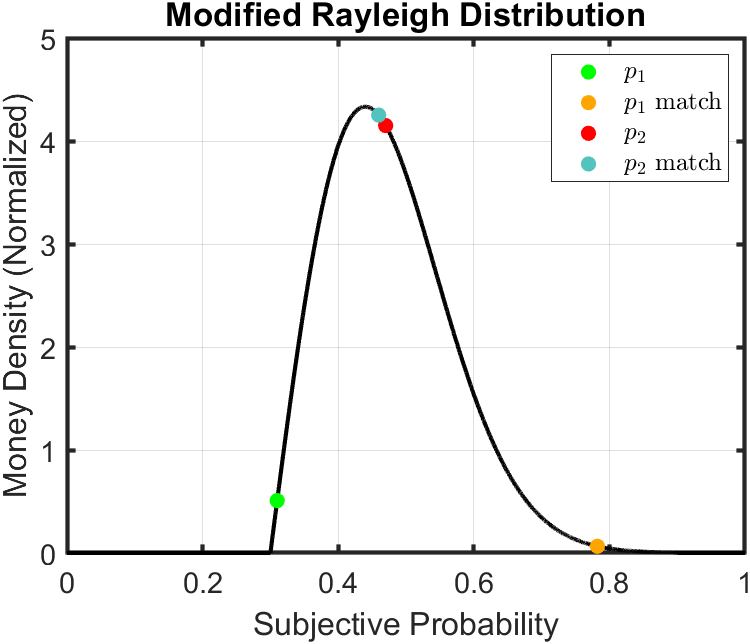
\includegraphics[width=10cm]{Rayleigh Distribution}
	\caption{Modified Rayliegh Distribution with Arbitrage}
\end{figure}

In the figure above, $p_1$ is set as low as possible, as the right skew ensures that $p_1 + \Gamma^{-1}(1-\Gamma(p_1))$ increases as $p_1$ decreases. As a result of the right skew, for any set of paired probabilities under an outside-in matching strategy, as the probability percentiles move away from the median, the probability at the higher percentile increases faster than the probability at the lower percentile decreases. In this case, the skew is pronounced enough to fulfill $p_1 + \Gamma^{-1}(1-\Gamma(p_1)) > 1$ at $p_1 = .31$, even though the median is below half unity, at .465. With the median at .465, $p_2$ is set just above the median, at $p_2 = .47$ so that the sum of it and its match remain belows 1. Thus, the conditions of Equations (30) and (31) are fulfilled, verifying that the opportunity for arbitrage exists. With $p_1$ set to .31 and $p_2$ set to .47, with respective betting amounts of $\$100$ and $\$95$, the profit from arbitrage comes out to roughly $\$9$, or a $4.6\%$ profit. 

That said, this arbitrage requires specific money density distributions. Across the $\mu \times \sigma$ mesh, across all subjective probabilities spaced from 0 to 1 in increments of .001, no arbitrage opportunities exist for solely peer bets. Furthermore, such arbitrage requires accurate knowledge of $\rho_M$ beforehand. While the $\rho_M$ distribution of previous batches could be conceivabely estimated by placing and analyzing bets, there is no guarantee that $\rho_M$ is static across time.

\subsection{Blended Arbitrage}

The second simple method of arbitrage involves a single (subjective probability, bet amount) pair whose peer bet and iterative money line bet have contradictory win conditions. As in the previous case of arbitrage, special characteristics of the batch's subjective probability and bet distributions can allow the payouts of each bet to exceed the stakes of the other bet. In this case, the subjective probability distribution has a median just past half unity, with minimal residual money for bets with subjective probabilities above the median. Since the median slice subjective probability is greater than half unity, a slice with probability just below the median will have a peer bet payoff ratio greater than 1. Since there is minimal residual money with subjective probabilities past the median, the $p_\alpha$ of the iterative money line is lowered below half unity, resulting in a money line bet on the focal outcome whose payoff greater than 1. As long as the stakes of both bets are roughly equivalent, the favorable payoff ratios and opposite win conditions guarantee arbitrage. Arbitrage is also possible for money density distributions centered just underneath half unity with minimal residual money below the median.

To verify this concept, I submitted a subjective probability of .499 and a bet amount of $\$9.75$ into a batch of 999 subjective probabilities and bet amounts. The 
batch subjective probabilities were randomly drawn from a modified beta distribution of $\mu = .505$, $\sigma = .03$ and the bet amounts were all set to $\$5$.
The first $\$5$ of the $\$9.75$ bet was engaged in a peer bet slice, which had a compliment win condition, a stake of $\$4.89$ and a payout of $\$4.94$. The remaining $\$4.86$ was bet through the iterative money line, which had a focal win condition, a stake of $\$4.86$ and a payout of $\$4.96$. No matter the binary event outcome, this arrangement guarantees at least $\$.07$ in profit. The different means of engagement for the bet amounts in this example are shown below as dependent on subjective probability. 

\begin{figure}[H]
	\centering
	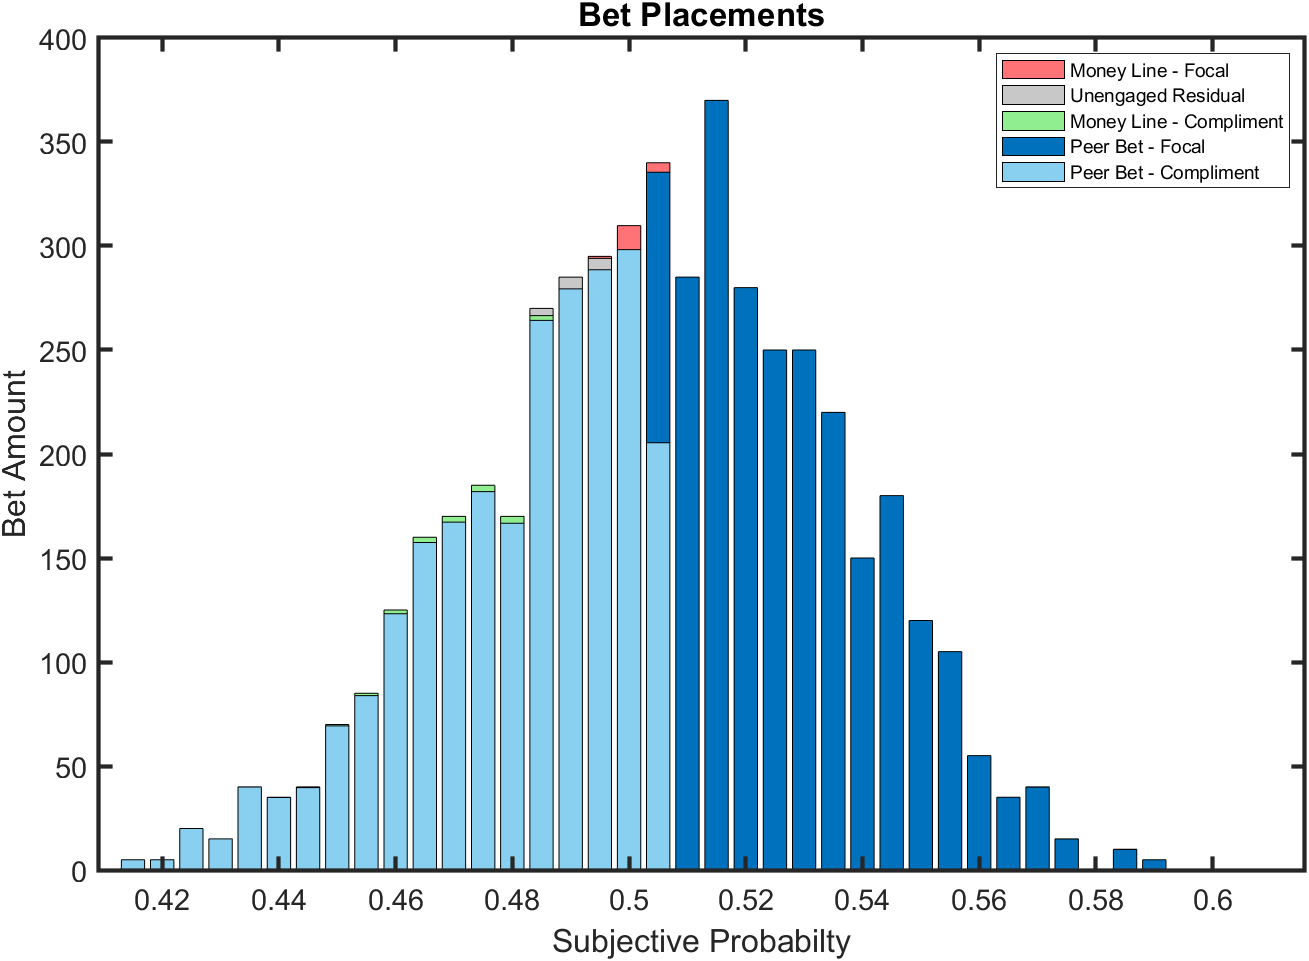
\includegraphics[width=13cm]{Bet Engagement Outcomes}
	\caption{Bet Engagement Distribution}
\end{figure}

\subsection{Summary}

I will end this section with a note that both of these arbitrage opportunities require special distributions of subjective probabilities and bet amounts. Both scenarios required the median slice subjective probability to be close to yet inequivalent to half unity. Peer bet arbitrage requires a significent skew past half unity. Blended arbitrage requires minimal residual betting amounts from users on the more extreme side of the median. As stated in Section 4, the subjective probability distribution is assumed to follow a modified beta distribution, with bet amounts drawn randomly from the interval $[\$0,\$100]$. These assumptions violate the requirements for both peer bet arbitrage and blended arbitrage. While more investigation is recommended to assess more complicated arbitrage bet portfolios, the opportunity for simple arbitrage in the synthesized speculation system is minimal. As a final consideration, slice sizes could be randomized between batches to limit the arbitrage opportunities that do exist.

% The Journal of Gambling Studies Uses an APA Style Format
\pagebreak
\begin{thebibliography}{9}

Action Network. (2019). Sportsbook Profit Margins. Sports Insights. https://www.sportsinsights.com/betting-tools/sportsbook-profit-margins/  \vspace{5pt}

\\Alós-Ferrer, C., \& Mihm, M. (2023). An Axiomatic Characterization of Bayesian Updating. Journal of Mathematical Economics, 104. https://doi.org/10.1016/j.jmateco.2022.102799 \vspace{5pt}

\\Andersen, S., Fountain, J., Harrison, G. W., \& Rutström, E. E. (2014). Estimating Subjective Probabilities. Journal of Risk and Uncertainty, 48(3), 207–229. https://doi.org/10.1007/s11166-014-9194-z \vspace{5pt}

\\Andrews, C. (2019). Then One Day... Huntington Press. \vspace{5pt}

\\BettorEdge. (2024). Frequently Asked Questions. https://www.bettoredge.com/faq \vspace{5pt}

\\Bickel, J. (2007). Some Comparison among Quadratic, Spherical, and Logarithmic Scoring Rules. Decision Analysis, 4(2), 49-65. https://doi.org/10.1287/deca.1070.0089 \vspace{5pt}

\\Dark Horse Odds. (2024). Arbitrage Betting. https://about.darkhorseodds.com/guides/sportsbook-arbitrage\vspace{5pt}

\\Eisenberg, E.,  \& Gale, D. (1959) Consensus of Subjective Probabilities: The Pari-Mutuel Method. Annals of Mathematical Statistics. 30(1), 165-168. https://doi.org/10.1214/aoms/1177706369 \vspace{5pt}
 
\\Goodman, L. A. (1960). On the Exact Variance of Products. Journal of the American Statistical Association, 55(292), 708-713. https://doi.org/10.2307/2281592 \vspace{5pt}

\\Heck, P., Simons, D., \& Chabris, C. (2018) $65\%$ of Americans Believe They Are Above Average In Intelligence: Results Of Two Nationally Representative Surveys. PLOS ONE 13(7). https://doi.org/10.1371/journal.pone.0200103 \vspace{5pt}

\\Hull, J. (2012). Options, Futures, and Other Derivatives. Prentice Hall.  \vspace{5pt}

\\Hurd, M. D. (2009). Subjective Probabilities in Household Surveys. Annual Review of Economics, 1, 543-562. \vspace{5pt}

\\Hurd, M. D., \& McGarry, K. (1993). Evaluation of Subjective Probability Distributions in the HRS. National Bureau of Economic Research Working Paper Series. Working Paper Number 4560. \vspace{5pt}

\\Levitt, S. D. (2004). Why Are Gambling Markets Organised So Differently From Financial Markets? The Economic Journal, 114, 223-246. https://doi.org/10.1111/j.1468-0297.2004.00207.x \vspace{5pt}

\\Maiter, D. (1985). The Psychology of Waiting Lines. The Service Encounter. Lexington Books. \vspace{5pt}

\\Malone, K., \& Herships, S. (2019, January 25). Episode 890: The Division Problem [Audio podcast episode]. Planet Money. NPR.  https://www.npr.org/sections/money/2019/01/25/688385893/episode-890-the-division-problem \vspace{5pt}

\\Markowitz, H. (1952) Portfolio Selection. The Journal of Finance, 7(1), 77-91. https://doi.org/10.1111/j.1540-6261.1952.tb01525.x \vspace{5pt}

\\Purdum, D. (2024). Exchanges Provide New Opportunities For American Bettors Of All Levels. ESPN. https://www.espn.com/chalk/story/_/id/34631766/exchanges-provide-new-opportunities-american-bettors-all-levels \vspace{5pt}

\\Quote Investigator. (2020). Quote Origin: No One in This World Has Ever Lost Money by Underestimating the Intelligence of the Great Masses of the Plain People. https://quoteinvestigator.com/2020/03/01/underestimate/ \vspace{5pt}

\\Rohatgi, V. K., \& Ehsanes Saleh, A. K. M. (2001). An Introduction to Probability and Statistics (2nd ed.). Wiley. \vspace{5pt}

\\Schwartz, D. G. (2006). Roll the Bones: The History of Gambling. Gotham Books. \vspace{5pt}

\\Schr\"{o}dinger, E. (1947). The Foundation of the Theory of Probability I. Proceedings of the Royal Irish Academy. Section A: Mathematical and Physical Sciences. 51. 51-66. \vspace{5pt}

\\Smith, J. (2002). Bookies Who Lose. http://www.betasia.com and reprinted from Business Life (March 2001). \vspace{5pt}

\\Su, F. E. (1999). Rental Harmony: Sperner's Lemma in Fair Division. The American Mathematical Monthly, 106(10), 930-942. \vspace{5pt}

\\Taroni, F., Garbolino, P., Biedermann, A., Aitken, C.,\& Bozza, S. (2018). Reconciliation of Subjective Probabilities and Frequencies in Forensic Science. Law, Probability and Risk, 17(3), 243-262. https://doi.org/10.1093/lpr/mgy012 \vspace{5pt}

\\von Holstein, C. S. (1971). The Effect of Learning on the Assessment of Subjective Probability Distributions. Organizational Behavior and Human Performance, 35(6), 304-315. https://doi.org/10.1016/0030-5073(71)90019-5 \vspace{5pt}

\\Walters, B. (2023). Gambler: A Life at Risk. Avid Reader Press. \vspace{5pt}

\\Wu, Y., Shih, W., \& Moore, D. (2008). Elicitation of a Beta Prior for Bayesian Inference in Clinical Trials. Biometrical Journal, 50(2), 212-223. https://doi.org/10.1002/bimj.200710390
\end{thebibliography}



\end{document}